%!TEX TS-program = xelatex
%!TEX encoding = UTF-8 Unicode


\documentclass{Dissertate}

\usepackage{tabularx}

\begin{document}
	
\renewcommand{\contentsname}{Indice}
\renewcommand{\listfigurename}{Elenco delle figure}
\renewcommand{\listtablename}{Elenco delle tabelle}

% the front matter
%!TEX root = ../dissertation.tex

% \maketitle
% \copyrightpage
\frontmatter
\setstretch{\dnormalspacing}
% \abstractpage
% \tableofcontents
% %\authorlist
% \listoffigures
% \dedicationpage
% \acknowledgments

% \doublespacing

\renewcommand{\figurename}{figura}
% include each chapter...
\setcounter{chapter}{0}  % start chapter numbering at 1
%!TEX root = ../dissertation.tex
\chapter{Introduzione}
\label{introduction}

Lorem ipsum dolor sit amet, consectetuer adipiscing elit. Morbi commodo, ipsum sed pharetra gravida, orci magna rhoncus neque, id pulvinar odio lorem non turpis. Nullam sit amet enim. Suspendisse id velit vitae ligula volutpat condimentum. Aliquam erat volutpat. Sed quis velit. Nulla facilisi. Nulla libero. Vivamus pharetra posuere sapien. Nam consectetuer. Sed aliquam, nunc eget euismod ullamcorper, lectus nunc ullamcorper orci, fermentum bibendum enim nibh eget ipsum. Donec porttitor ligula eu dolor. Maecenas vitae nulla consequat libero cursus venenatis. Nam magna enim, accumsan eu, blandit sed, blandit a, eros.

%!TEX root = ../dissertation.tex
% For an example of a full page figure, see Fig.~\ref{fig:myFullPageFigure}.

\chapter{Contesto aziendale}

\section{L'azienda}
Lo stage si è svolto presso l'azienda Pietro Fiorentini S.p.A nella sede principale di Arcugnano. Pietro Fiorentini realizza prodotti e servizi tecnologicamente avanzati per la distribuzione e l'utilizzo del petrolio e del gas naturale a livello globale, con undici stabilimenti nel mondo.
L'azienda realizza prodotti come valvole, filtri, regolatori di pressione, ma lo stage si è interessato in particolare sui Multiphase Flow Meter.

\section{Multiphase Flow Meter} \label{multiphaseflowmeter}
Un Multiphase Flow Meter, o MPFM in breve, è un dispositivo utilizzato per misurare le singole portate delle fasi costitutive di un determinato flusso. In questo caso il flusso è una miscela di petrolio, acqua e gas creata durante il processo di estrazione dal pozzo petrolifero.
I MPFM prodotti dalla Pietro Fiorentini sono strumenti non intrusivi per effettuare misurazioni in tempo reale del flusso evitando l'uso di sistemi basati sulla separazione delle diverse fasi.
Gli MPFM sono modulari e possono essere installati in diverse configurazioni, ogni modulo si occupa di effettuare una o più misurazioni sul flusso.

La misurazione dei flussi multifase è un problema complesso e richiede la considerazione di molte possibili condizioni. In particolare ci sono molti regimi di scorrimento del flusso a seconda della velocità delle parti liquide e gassose \cite{multiphaseIntroduction}.

I principali regimi di scorrimento sono:

\begin{itemize}
	\item{Bubble}: il gas è sospeso in bollicine all'interno del liquido, accade quando la parte liquida è più veloce di quella gassosa.
	\item{Finely dispersed bubble}: il gas è sospeso in bollicine molto piccole all'interno del liquido.
	\item{Slug}: il flusso è a intermittenza prevalentemente liquido e prevalentemente gassoso, formando delle grosse bolle di gas.
	\item{Churn}: all'aumentare della velocità del gas il flusso diventa irregolare e la parte liquida sale e scende continuamente.
	\item{Annular}: ad alte velocità del gas la parte liquida forma un anello intorno alle pareti della tubatura, e il gas scorre nel centro.
\end{itemize}

\begin{figure}
	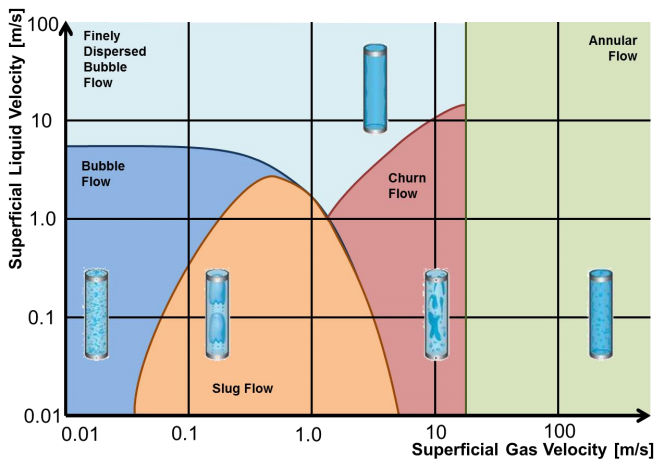
\includegraphics[width=\textwidth]{figures/flowtypes}
	\caption[Tipologie di flusso multifase]{
		I principali regimi di scorrimento del flusso multifase in base alla velocità della parte liquida e della parte gassosa \cite{multiphaseIntroduction}.
		\label{fig:flowtypes}}
\end{figure}

L'irregolarità del flusso rende anche più difficile il riconoscimento delle anomalie nel funzionamento dello strumento. Dei valori che a prima vista sembrano anomali potrebbero semplicemente essere delle bolle più grosse di gas, oppure il passaggio improvviso a un altro regime di scorrimento. In questi casi le anomalie registrate fanno parte del funzionamento corretto dello strumento e non devono essere quindi considerati come valori anormali.

\section{Struttura dei dati} \label{"StrutturaDeiDati"}
I dati rilevanti al progetto riguardano una serie di test effettuati in vari laboratori negli ultimi dieci anni. I test consistono nell'uso di un Multiphase Flow Meter in un circuito chiuso, in modo da poter controllare accuratamente la composizione e le condizioni del flusso che viene fatto circolare. 

Durante il test si registrano le letture di tutti i sensori presenti nel MPFM, questi dati vengono quindi salvati in file singoli, ognuno dei quali contiene in genere un minuto di lettura. I file sono in formato proprietario BIN o BIX e rappresentano i dati nel loro stato "raw", ad esempio un sensore che misura la pressione non salverà direttamente dei valori in atmosfere ma potrebbe salvare dei voltaggi che dovranno essere a loro volta interpretati.

Le informazioni sulla configurazione del MPFM e sulle condizioni del flusso non sono salvate nei file raw, sono salvate invece in file separati, rispettivamente un file di testo per la configurazione del MPFM e un foglio di calcolo per le condizioni del flusso. Questo foglio di calcolo, chiamato anche foglio di riferimento, rappresenta quindi le condizioni in cui sono state effettuate le letture dei sensori, in particolare descrive le seguenti proprietà del flusso per ogni file raw:

\begin{itemize}
	\item \bfseries{Qgas}: Il volume della componente di gas nel flusso
	\item \bfseries{Qwater}: Il volume della componente d'acqua nel flusso
	\item \bfseries{Qwater}: Il volume della componente di petrolio nel flusso
	\item \bfseries{WLR}: Water Liquid Ratio, la percentuale di acqua sul totale del liquido. Calcolato con la formula: \[\frac{Qwater}{Qwater+Qoil}\]
	\item \bfseries{GVF}: Gas Volume Fraction, la frazione di gas sul volume totale. Calcolato con la formula: \[\frac{Qgas}{Qwater+Qoil+Qgas}\]
	\item \bfseries{Pressure}: La pressione del flusso
	\item \bfseries{Temperature}: La temperatura del flusso
\end{itemize}




%% Requires fltpage2 package
%%
% \begin{FPfigure}
% 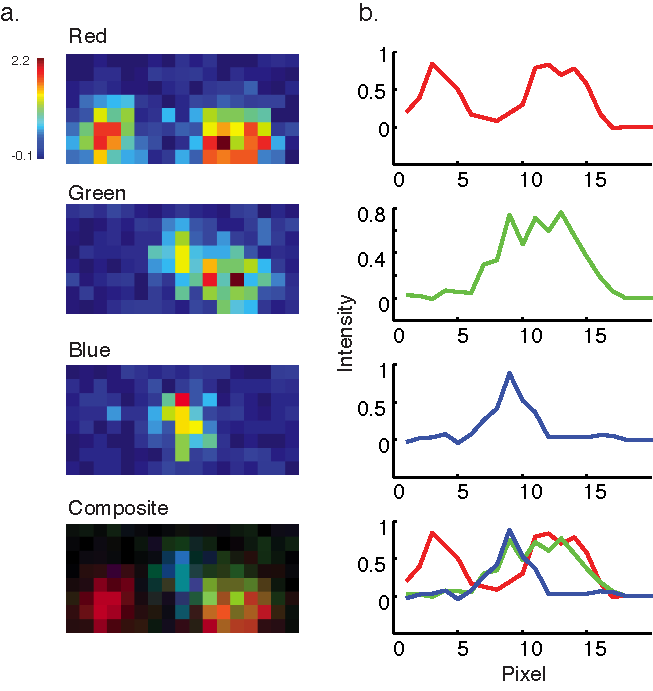
\includegraphics[width=\textwidth]{figures/fullpage}
% \caption[Short figure name.]{This is a full page figure using the FPfigure command. It takes up the whole page and the caption appears on the preceding page. Its useful for large figures. Harvard's rules about full page figures are tricky, but you don't have to worry about it because we took care of it for you. For example, the full figure is supposed to have a title in the same style as the caption but without the actual caption. The caption is supposed to appear alone on the preceding page with no other text. You do't have to worry about any of that. We have modified the fltpage package to make it work. This is a lengthy caption and it clearly would not fit on the same page as the figure. Note that you should only use the FPfigure command in instances where the figure really is too large. If the figure is small enough to fit by the caption than it does not produce the desired effect. Good luck with your thesis. I have to keep writing this to make the caption really long. LaTex is a lot of fun. You will enjoy working with it. Good luck on your post doctoral life! I am looking forward to mine. \label{fig:myFullPageFigure}}
% \end{FPfigure}
% \afterpage{\clearpage}

%!TEX root = ../dissertation.tex

\chapter{Il progetto di stage}
Pietro Fiorentini sta sviluppando un sistema di auto-diagnostica per i Multiphase Flow Meter, con l'obiettivo di avere sistemi sempre più intelligenti che riescano a dare informazioni relativamente al loro stato di funzionamento e salute. 
I dati raccolti da vari sensori presenti nei MPFM sono analizzati attraverso algoritmi di machine learning per identificare automaticamente eventuali anomalie o malfunzionamenti.
Il progetto include la creazione di adeguate infrastrutture software per la gestione dei dati e la loro analisi, per poi poter applicare e valutare gli algoritmi di machine learning.

\section{Piano di lavoro}
Lo stage segue un piano di lavoro redatto prima dell'inizio dello stage dal tutor aziendale in collaborazione con lo stagista e approvato dal tutor universitario.
Il piano di lavoro definisce gli obiettivi di ogni settimana di stage.

\subsection{Settimana 1 - Analisi dei requisiti}

\begin{itemize}
	\item Incontro con persone coinvolte nel progetto Machine Learning per discutere i requisiti e le richieste relativamente al progetto e alla qualità del software
	\item Verifica credenziali e strumenti di lavoro assegnati
	\item Presa visione dell'infrastruttura esistente
	\item Analisi dei requisiti, tenendo in considerazione il preesistente
	\item Discussione e redazione del documento del "Requirement Specification"
\end{itemize}
Risultato: Documento "Requirement Specification" che raccoglie tutti i vincoli e requisiti del progetto.

\subsection{Settimana 2 e 3 - Gestione dei dati}

\begin{itemize}
	\item Studio dei dati e delle informazioni a corredo (quando sono stati raccolti, dove, con quale strumento)
	\item Studio delle infrastrutture per gestire i dati (DB, Data Warehouse, Data Lake, etc)
	\item Creare struttura per gestire e  accedere facilmente ai dati, combinando tutte le informazioni disponibili
\end{itemize}
Risultato: Documento che spiega come implementare una infrastruttura per la gestione dei dati "Data Management Design" e l’infrastruttura software per la gestione dei dati.

\subsection{Settimana 4 e 5 - Analisi dei dati}

\begin{itemize}
	\item Studio del formato con cui sono salvati i dati (non standard, proprietario)
	\item Librerie in Python per accedere al contenuto dei dati e poterli analizzare
	\item Creare la struttura software per estrarre le informazioni dai dati e per creare grafici e analizzarli
	\item Strumento o interfaccia per visualizzare e analizzare dati ricavati da fonti diverse
\end{itemize}
Risultato: Documento "Data Analytics Design" che descriva come implementare la lettura dei dati grezzi, creare grafici e analizzarli, creazione del software per interfacciarsi con i dati.

\subsection{Settimana 6 - Feature extraction}

\begin{itemize}
	\item Studio di metodi per estrazione di caratteristiche dai dati e metriche per il confronto dei metodi, con lo scopo di rendere più semplice l’individuare anomalie
	\item Implementazione e confronto dei vari metodi per estrarre caratteristiche
\end{itemize}
Risultato: Documento "Feature Extraction Design \& Report" che descriva i metodi di estrazione e il loro confronto e valutazione, creazione del software con i metodi implementati.

\subsection{Settimana 7 - Anomaly detection}

\begin{itemize}
	\item Studio di modelli e algoritmi di machine learning per la rilevazione di anomalie, studio di metriche per il confronto
	\item Valutazione e confronto dei modelli sui dati per identificare anomalie sulla base di metriche prestabilite
\end{itemize}
Risultato: Documento "Anomaly Detection Design \& Report" che descriva gli algoritmi di identificazione anomalie, il loro confronto e valutazione, creazione del software con gli algoritmi implementati

\subsection{Settimana 8 - Conclusione}

\begin{itemize}
	\item Incontro con il team di Ricerca e Sviluppo per presentare e insegnare ad usare quanto prodotto
	\item Live-demo di tutto il lavoro di stage
\end{itemize}
Risultato: Presentazione e live-demo

\section{Obiettivi}

\subsection{Obiettivi minimi}
Documenti:
\begin{itemize}
	\item Requirement Specification: sezione "General Requirement"
	\item Data Management Design: diagramma a blocchi dell'infrastruttura
	\item Data Analytics Design: diagramma a blocchi dell'infrastruttura
	\item Feature Extraction Design \& Report: descrizione di un solo metodo di
	feature extraction
	\item Anomaly Detection Design \& Report: due algoritmi di anomaly detection descritti e valutati
	\item Presentazione finale
\end{itemize}
Software:
\begin{itemize}
	\item Database di gestione dei dati
	\item Software per l'analisi dei dati (script per accedere ai dati)
	\item Software per feature extraction, un solo metodo implementato
	\item Software per anomaly detection, implementazione, confronto e valutazione di due algoritmi
\end{itemize}

\subsection{Obiettivi desiderabili}
Tutti gli obiettivi minimi con le seguenti aggiunte o modifiche.

Documenti:
\begin{itemize}
	\item Requirement Specification completo di informazioni per verificare e testare i
	requisiti
	\item Data Management Design completo
	\item Data Analytics Design completo
	\item Feature Extraction Design \& Report: descrizione di tre metodi di feature extraction, valutazione e confronto
	\item Anomaly Detection Design \& Report: descrizione di cinque algoritmi di anomaly detection, valutazione e confronto
	\item Presentazione finale e dimostrazione live del software sviluppato su un set di dati
\end{itemize}
Software:
\begin{itemize}
	\item Infrastruttura di gestione dati completamente implementata
	\item Software per l'analisi dei dati completamente implementato
	\item Software per feature extraction, confronto e valutazione di tre metodi
	\item Software per anomaly detection, confronto e valutazione di cinque algoritmi
\end{itemize}


\section{Vincoli}
Il progetto deve rispettare dei determinati vincoli imposti dall'azienda o dall'università

\subsection{Vincoli temporali}
L'università impone un vincolo temporale minimo di 300 ore di lavoro durante lo stage. Per questo motivo il progetto è stato diviso in 8 settimane, lavorando 40 ore a settimana per un totale massimo di 320 ore.

\subsection{Vincoli metodologici}
I documenti, il codice e i commenti scritti durante il progetto devono essere completamente in inglese.

Tutto ciò che viene prodotto durante lo stage deve essere versionato nel repository Git fornito dall'azienda.

L'azienda non ha definito altri vincoli metodologici, e ha dato libera scelta per gli strumenti di sviluppo. Come IDE è stato utilizzato PyCharm essendo uno degli IDE più completi per lo sviluppo in Python. GitKraken è stato usato come client di Git per facilitare il lavoro condiviso attraverso il repository fornito. Per la documentazione del codice è stato usato Sphinx, in modo da generare la documentazione automaticamente a partire dai commenti presenti nel codice.

\subsection{Vincoli tecnologici}
L'utilizzo di Python 3 come linguaggio di programmazione è stato fortemente consigliato dall'azienda vista la presenza di molte librerie per la visualizzazione dei dati e l'applicazione di feature extraction e anomaly detection.

La scelta del database è stata libera, ma MySql è stato preferito in quanto già installato e funzionante all'interno dell'azienda.


%!TEX root = ../dissertation.tex
\chapter{Analisi dei requisiti}

Questo capitolo descrive i requisiti individuati per soddisfare tutti gli obiettivi definiti nel piano di lavoro.
I requisiti descrivono in modo chiaro tutte le funzionalità del sistema finale senza entrare in dettagli implementativi o vincolare l'uso di specifiche librerie o framework.


\section{Casi d'uso}
I casi d'uso riportati sono emersi nella prima settimana di lavoro, in base al piano di lavoro stabilito precedentemente e alle informazioni fornite dal responsabile aziendale. 
Questi casi d'uso forniscono una panoramica di tutte le funzionalità che dovrà avere il sistema completo.

L'unico attore è l'utente o user, ovvero colui che utilizza il sistema. Nel contesto aziendale sarà uno dei ricercatori che vuole analizzare o effettuare altre operazioni sui dati.



\subsection{Gestione dei dati}

\begin{figure} [H]
	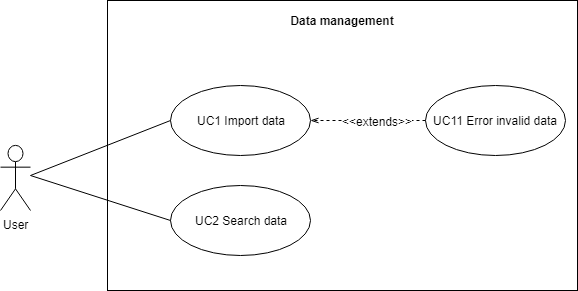
\includegraphics[width=\textwidth]{figures/UCDataManagement}
	\caption[Panoramica casi d'uso gestione dei dati]{
		Panoramica dei casi d'uso del sistema di gestione dei dati.
		\label{fig:UCDataManagement}}
\end{figure}

\begin{itemize}
	\item UC1 Import data: l'utente può importare nuovi dati nel sistema di gestione dati
	\item UC2 Search data: l'utente può cercare particolari dati in base a una condizione data, il risultato viene ritornato per poter essere analizzato in seguito
	\item UC11 Error invalid data: l'utente viene informato se i dati importati non sono nel formato corretto
\end{itemize}


\begin{figure} [H]
	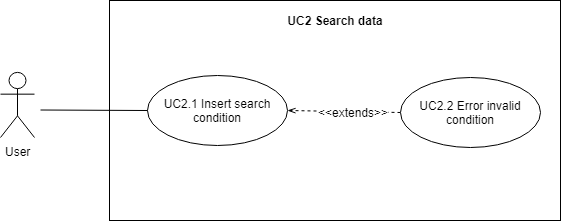
\includegraphics[width=\textwidth]{figures/UC2}
	\caption[Caso d'uso UC2]{
		Sottocasi d'uso di UC2.
		\label{fig:UC2}}
\end{figure}

\begin{itemize}
	\item UC2.1 Insert search condition: l'utente può specificare una condizione di ricerca che include uno o più dei seguenti parametri dei dati:
	\begin{itemize}
		\item \bfseries{Qgas}: Il volume della componente di gas nel flusso
		\item \bfseries{Qwater}: Il volume della componente d'acqua nel flusso
		\item \bfseries{Qwater}: Il volume della componente di petrolio nel flusso
		\item \bfseries{WLR}: Water Liquid Ratio, la percentuale di acqua sul totale del liquido
		\item \bfseries{GVF}: Gas Volume Fraction, la frazione di gas sul volume totale
		\item \bfseries{Pressure}: La pressione del flusso
		\item \bfseries{Temperature}: La temperatura del flusso
		\item \bfseries{Modules}: Quale dei moduli era installato il momento della lettura dei dati
		\item \bfseries{Time}: La data e l'orario di lettura dei dati
		\item \bfseries{Place}: Il luogo in cui sono stati letti i dati
	\end{itemize}

	\item UC2.2 Error invalid condition: l'utente viene informato se la condizione inserita non è formattata correttamente
\end{itemize}

\subsection{Analisi dei dati}


\begin{figure} [H]
	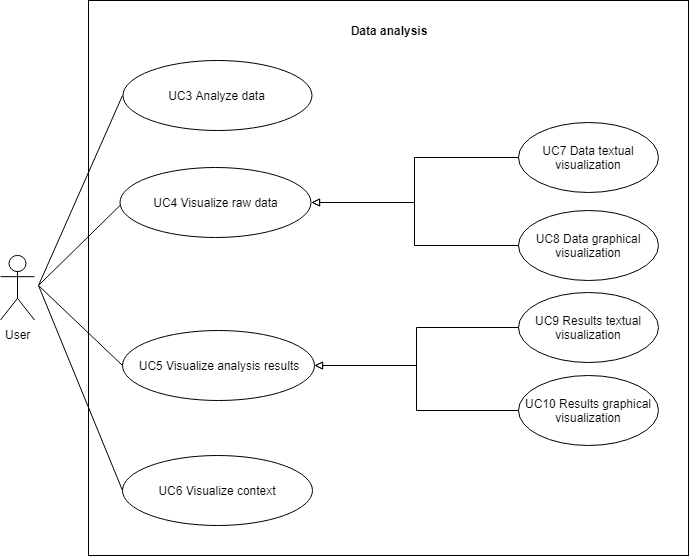
\includegraphics[width=\textwidth]{figures/UCDataAnalysis}
	\caption[Panoramica casi d'uso analisi dei dati]{
		Panoramica dei casi d'uso del sistema di analisi dei dati.
		\label{fig:UCDataAnalysis}}
\end{figure}

\begin{itemize}
	\item UC3 Analyze data: l'utente può applicare un metodo di analisi dei dati, il risultato è adatto alla visualizzazione grafica e testuale
	\item UC4 Visualize raw data: l'utente può visualizzare i dati originali
	\item UC5 Visualize analysis results: l'utente può visualizzare il risultato dell'analisi
	\item UC6 Visualize context: l'utente può accedere a tutti i documenti relativi ai dati, ad esempio file di setup, file excel di riferimento, note del laboratorio
	\item UC7 Data textual visualization: l'utente può visualizzare i dati in un formato testuale
	\item UC8 Data graphical visualization: l'utente può visualizzare i dati in un formato grafico
	\item UC9 Results textual visualization: l'utente può visualizzare i risultati dell'analisi in un formato testuale
	\item UC10 Results graphical visualization: l'utente può visualizzare i risultati dell'analisi in un formato grafico
\end{itemize}

\begin{figure} [H]
	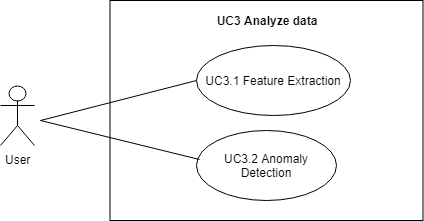
\includegraphics[width=\textwidth]{figures/UC3}
	\caption[Caso d'uso UC3]{
		Sottocasi d'uso di UC3.
		\label{fig:UC3}}
\end{figure}

\begin{itemize}
	\item UC3.1 Feature extraction: l'utente può applicare il metodo di "Feature extraction" desiderato
	\item UC3.2 Anomaly detection: l'utente può applicare il metodo di "Anomaly detection" desiderato
	
\end{itemize}

\section{Requisiti}
\subsection{Classificazione dei requisiti}
Tutti i requisiti sono classificati in base alla tipologia, alla priorità e alla fonte. Ogni requisito è inoltre associato a un codice identificativo univoco.

Le possibili tipologie sono:
\begin{itemize}
	\item GR: General Requirements, per i requisiti generali sul funzionamento
	\item SR: System Requirements, per i requisiti che riguardano le caratteristiche del sistema
	\item QR: Quality Requirements, per i requisiti di qualità
	\item DOC: Documentation, per i requisiti che riguardano la documentazione
\end{itemize}
Le possibili priorità sono:
\begin{itemize}
	\item Obbligatorio
	\item Desiderabile
	\item Opzionale
\end{itemize}
Le possibili fonti sono:
\begin{itemize}
	\item PF: Pietro Fiorentini
	\item Interno
\end{itemize}


\subsection{Requisiti generali}
\begin{table} [H]
	\centering
	\begin{tabularx}{\textwidth}{|c c X c|} 
		\hline
		ID & Priorità & Requisito & Fonte \\ [0.5ex] 
		\hline\hline
		\texttt{GR-001} & Obbligatorio & L'utente può importare nuovi dati nel sistema & PF \\ 
		\hline
		\texttt{GR-002} & Obbligatorio & L'utente può cercare particolari dati in base a una condizione data & PF \\ 
		\hline
		\texttt{GR-003} & Desiderabile & L'utente può applicare un qualunque metodo di analisi al risultato della ricerca & PF \\ 
		\hline
		\texttt{GR-004} & Obbligatorio & L'utente può applicare il metodo di feature extraction desiderato & PF \\ 
		\hline
		\texttt{GR-005} & Obbligatorio & L'utente può applicare il metodo di anomaly detection desiderato & PF \\ 
		\hline
		\texttt{GR-006} & Obbligatorio & L'utente può visualizzare i dati in un formato testuale & PF \\ 
		\hline
		\texttt{GR-007} & Desiderabile & L'utente può visualizzare i dati in un formato grafico & PF \\ 
		\hline
		\texttt{GR-008} & Obbligatorio & L'utente può visualizzare i dati risultanti da un'analisi in un formato testuale & PF \\ 
		\hline
		\texttt{GR-009} & Desiderabile &L'utente può visualizzare i dati risultanti da un'analisi in un formato grafico & PF \\ 
		\hline
		\texttt{GR-010} & Desiderabile & L'utente può accedere a tutti i documenti contestuali relativi ai dati ricercati & PF \\ 
		\hline
		\texttt{GR-011} & Obbligatorio & Il sistema deve offrire un'interfaccia per cercare e ritornare i file richiesti & PF \\ 
		\hline
		\texttt{GR-012} & Obbligatorio & Il sistema deve offrire un'interfaccia per accedere al contenuto dei file richiesti & PF \\ 
		\hline
		\texttt{GR-013} & Obbligatorio & Il sistema è in grado di leggere e utilizzare il contenuto dei file BIN e BIX & PF \\ 
		\hline
		\texttt{GR-014} & Opzionale & Il sistema è in grado di leggere e utilizzare il contenuto dei file txt e xls & PF \\ 
		\hline

	\end{tabularx}
	\caption{Tabella dei requisiti generali}
\end{table}


\subsection{Requisiti di sistema}
\begin{table} [H]
	\centering
	\begin{tabularx}{\textwidth}{|c c X c|} 
		\hline
		ID & Priorità & Requisito & Fonte \\ [0.5ex] 
		\hline\hline
		\texttt{SR-001} & Desiderabile & Il sistema è sviluppato in Python & PF \\ 
		\hline
		\texttt{SR-002} & Desiderabile & Il sistema funziona in un sistema operativo Linux & PF \\ 
		\hline
		
	\end{tabularx}
	\caption{Tabella dei requisiti di sistema}
\end{table}

\subsection{Requisiti di qualità}
\begin{table} [H]
	\centering
	\begin{tabularx}{\textwidth}{|c c X c|} 
		\hline
		ID & Priorità & Requisito & Fonte \\ [0.5ex] 
		\hline\hline
		\texttt{QR-001} & Obbligatorio & Il codice segue lo stile guida definito in PEP8 & Interno \\ 
		\hline
		
	\end{tabularx}
	\caption{Tabella dei requisiti di qualità}
\end{table}

\subsection{Documentazione}
\begin{table} [H]
	\centering
	\begin{tabularx}{\textwidth}{|c c X c|} 
		\hline
		ID & Priorità & Requisito & Fonte \\ [0.5ex] 
		\hline\hline
		\texttt{DOC-001} & Obbligatorio & Stesura del documento "Requirements Specification" & PF \\ 
		\hline
		\texttt{DOC-002} & Obbligatorio & Stesura del documento "Data Management Design" & PF \\ 
		\hline
		\texttt{DOC-003} & Obbligatorio & Stesura del documento "Data Analytics Design" & PF \\ 
		\hline
		\texttt{DOC-004} & Obbligatorio & Stesura del documento "Feature Extraction Design \& Report" & PF \\ 
		\hline
		\texttt{DOC-005} & Obbligatorio & Stesura del documento "Anomaly Detection Design \& Report" & PF \\ 
		\hline
	\end{tabularx}
	\caption{Tabella dei requisiti sulla documentazione}
\end{table}


%!TEX root = ../dissertation.tex
\chapter{Gestione dei dati}


Prima di analizzare i dati è importante poter trovarli in modo efficiente ed efficace. Questo capitolo descrive i sistemi software implementati per la gestione dei dati, incluse operazioni come la ricerca rapida di specifici file raw in base a una o più condizioni, ma non affronta la lettura dei file stessi.

I file raw sono associati ai metadati disponibili nel foglio di calcolo di riferimento e nel file di configurazione del MPFM. Ogni file inoltre contiene nel nome la data in cui è stato creato nel formato \texttt{"YYYYmmdd hhmm"}

\section{Archiettura generale}
L'architettura del sistema di gestione dei dati può essere divisa in due parti principali. La prima parte si occupa di trovare e leggere i file di riferimento e configurazione per associare i metadati ai corretti file raw. La seconda parte si occupa di caricare tutte le informazioni raccolte in un database, per poter effettuare ricerche più complesse e veloci.
Navigare il sistema operativo esaustivamente per trovare tutti i file interessati è un'operazione temporalmente costosa, nell'ordine di una decina di minuti per le cartelle più grandi presenti nel server. Per migliorare il tempo di esecuzione vengono ricercati contemporaneamente tutti i tipi di file necessari, sia raw che di riferimento, invece di dover ripetere l'esplorazione più volte.
La ricerca deve essere sempre completa di tutte le sottocartelle in quanto i dati arrivano da molti laboratori diversi e la posizione dei file non rispetta uno standard uniforme.


\begin{figure}
	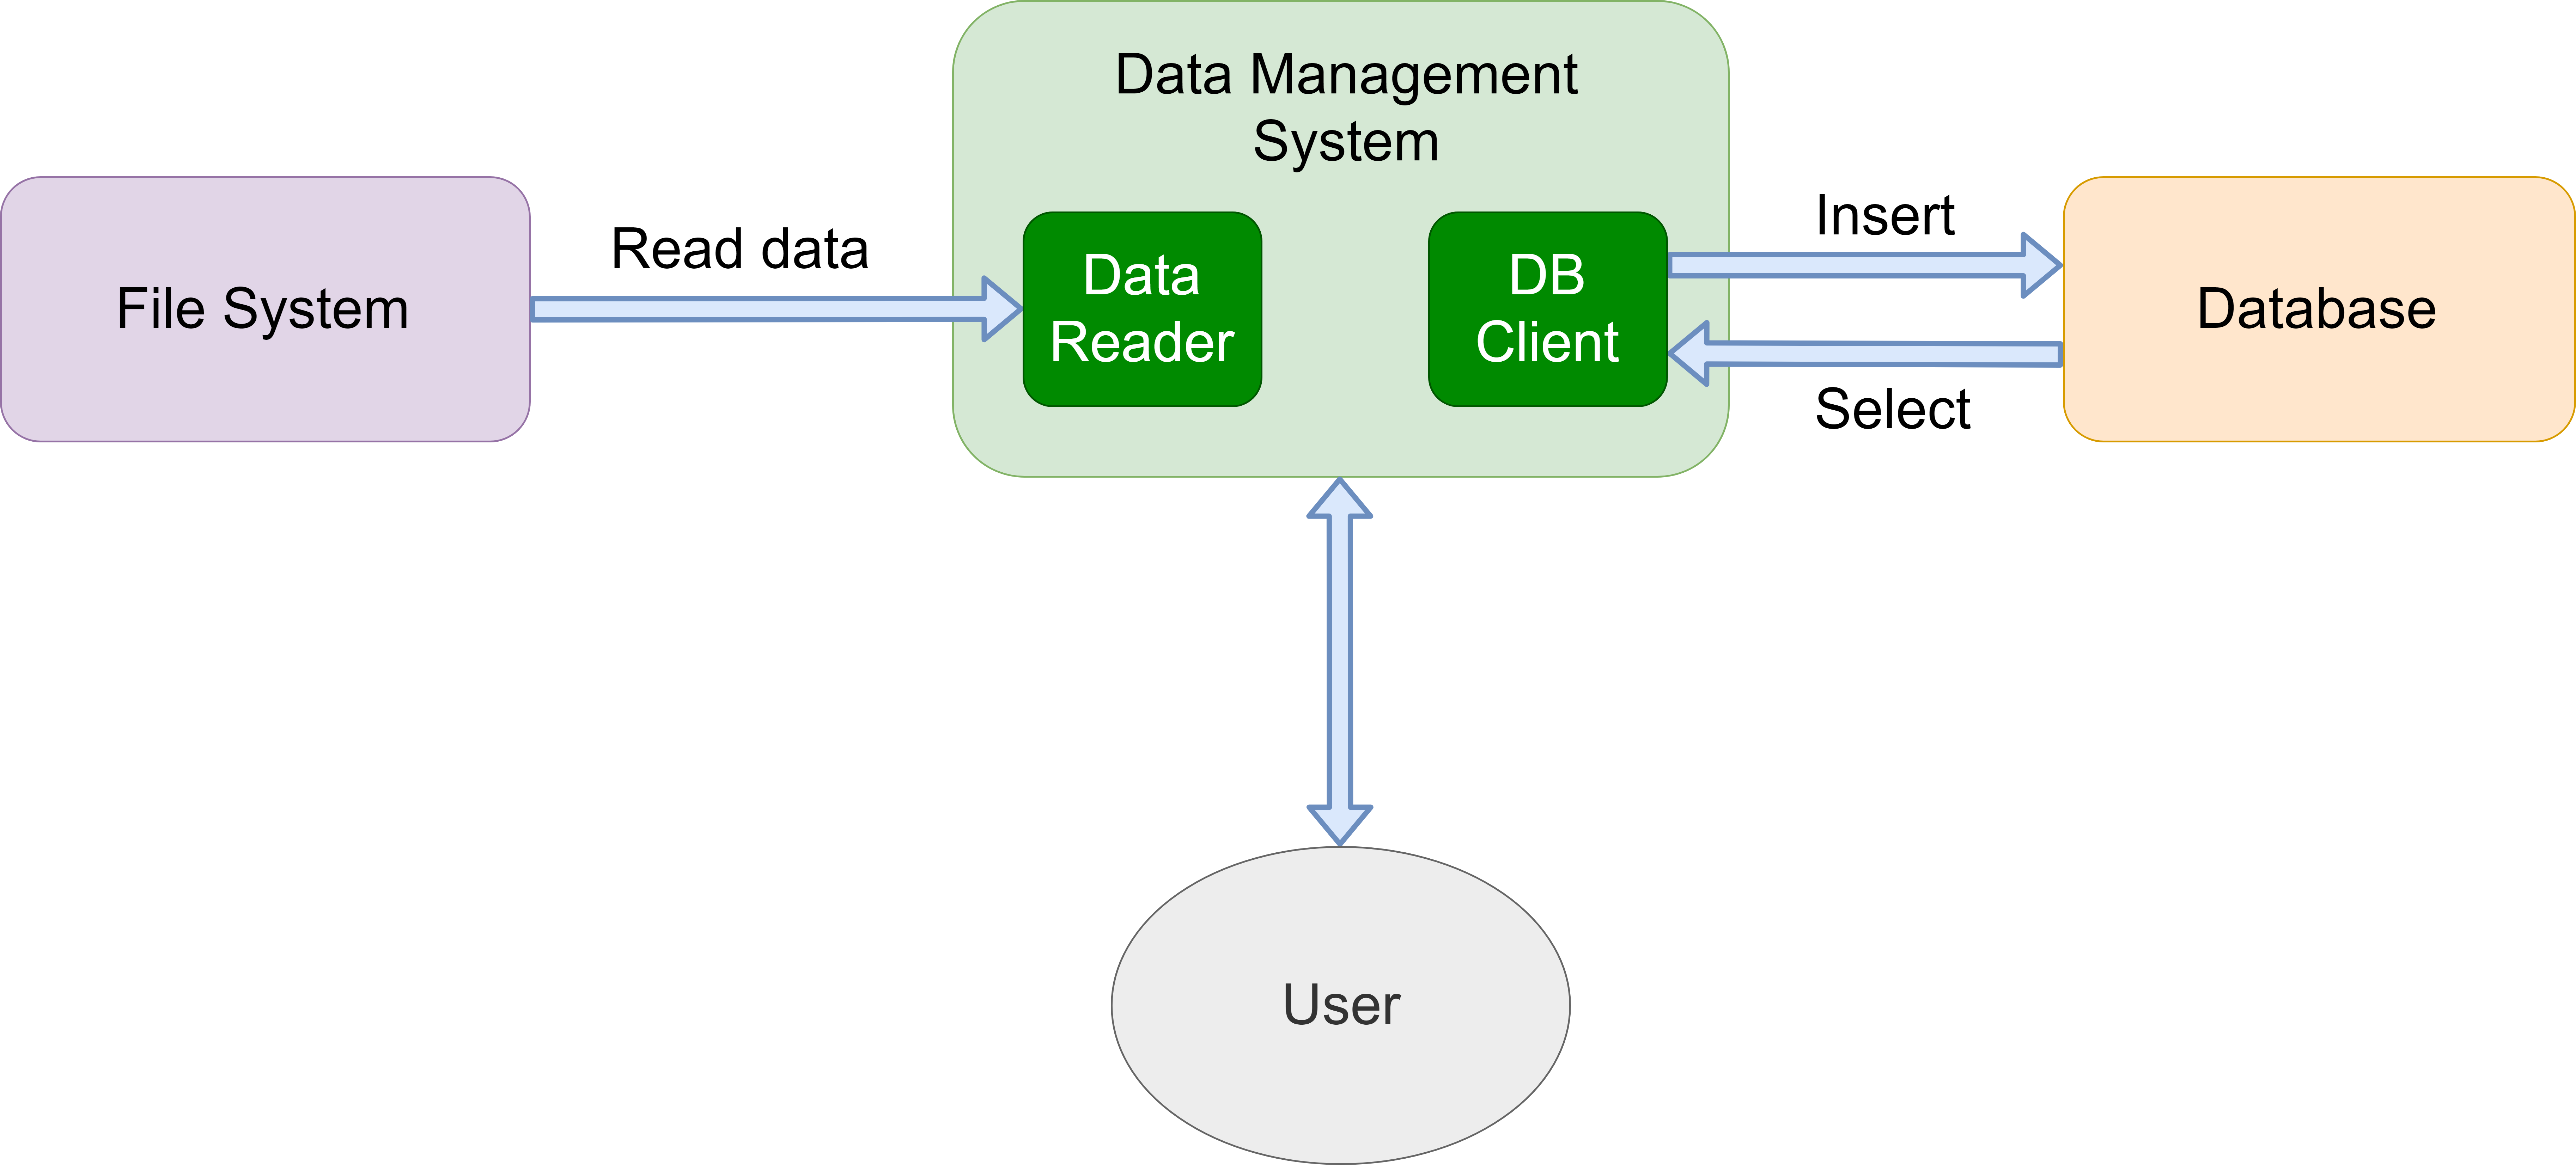
\includegraphics[width=\textwidth]{figures/ArchitetturaDMD}
	\caption[Architettura sistema di gestione dei dati]{Architettura generale del sistema di gestione dei dati e le interazioni verso le componenti esterne al sistema. 
		\label{fig:ArchietturaDMD}}
\end{figure}

\section{Diagramma delle classi} \label{DiagrammaDelleClassiDMD}

\begin{figure}
	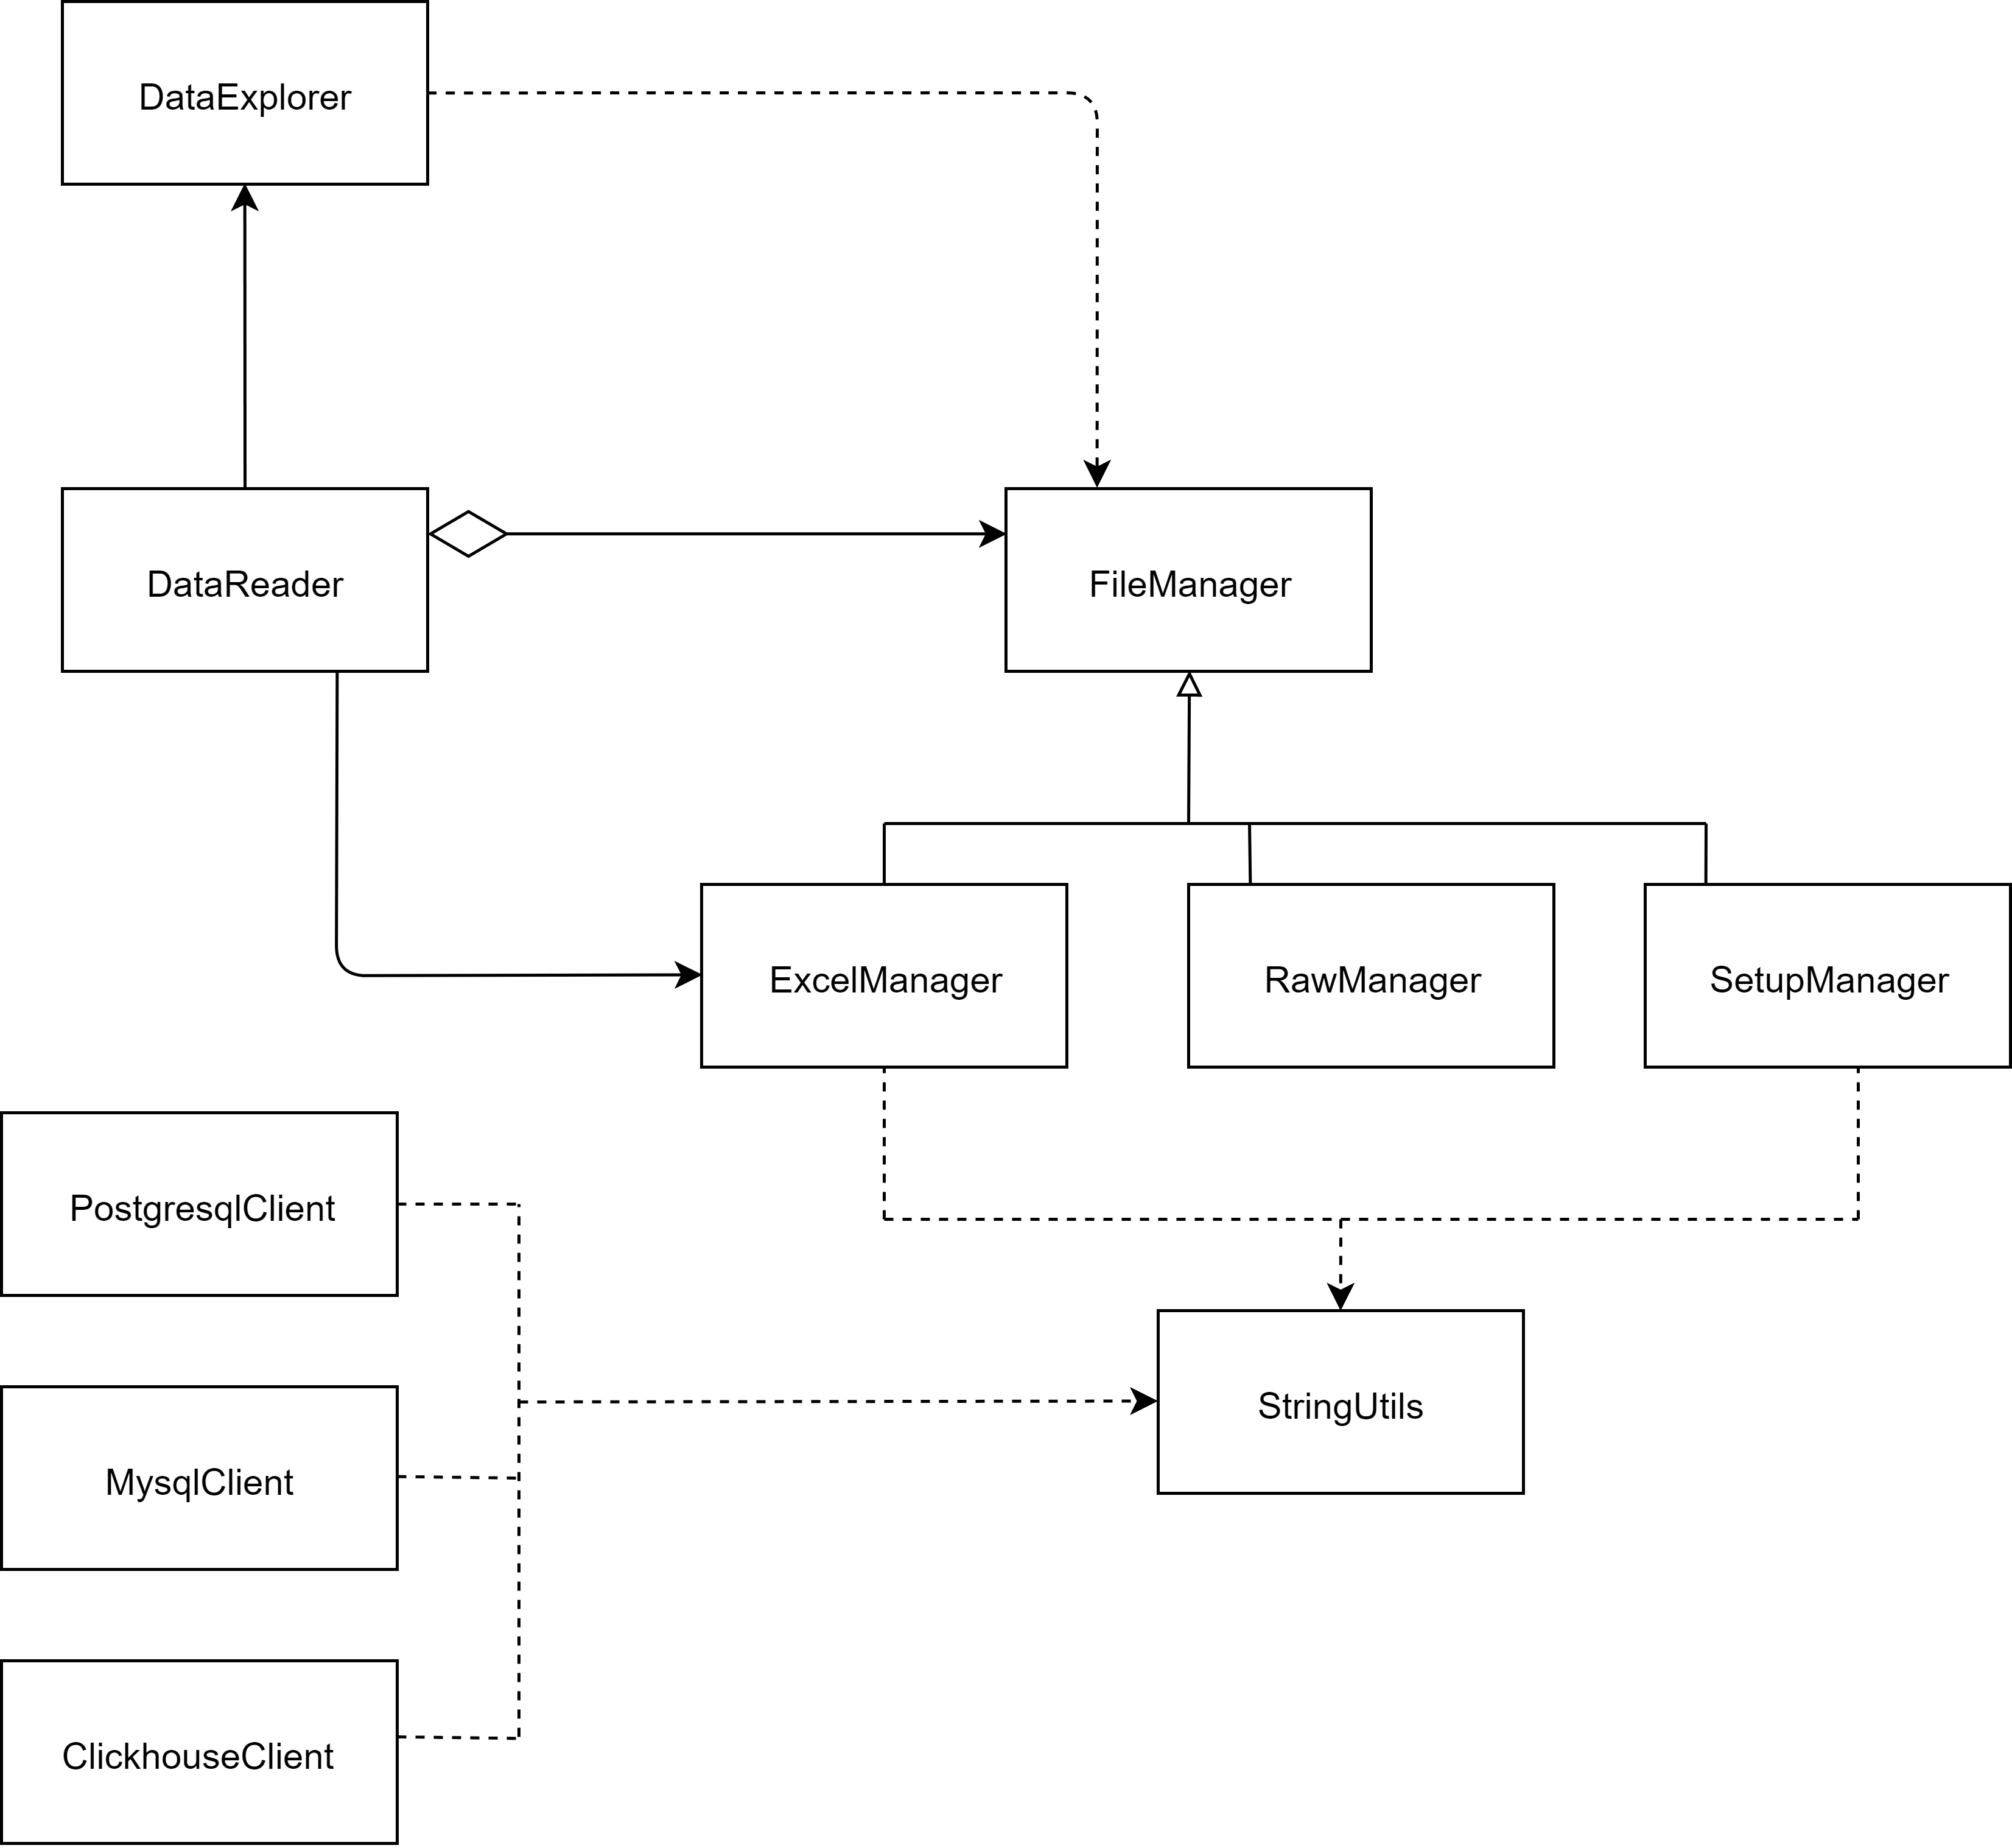
\includegraphics[width=\textwidth]{figures/DiagrammaDelleClassiDMD}
	\caption[Diagramma delle classi sistema di gestione dei dati]{Diagramma delle classi generale del sistema di gestione dei dati, rappresenta le dipendenze tra le classi senza entrare nei dettagli implementativi. 
		\label{fig:DiagrammaDelleClassiDMD}}
\end{figure}


DataReader è la classe principale del sistema di gestione dati e offre tutte le funzionalità necessarie per trovare i file e associarli con i relativi metadati.

ExcelManager, RawManager e SetupManager sono tre classi che gestiscono rispettivamente i file excel, i file raw, e file di testo di setup. Ognuno di questi Manager implementa due metodi fondamentali:

\begin{itemize}
	\item il metodo \texttt{match()} che dato il percorso e il nome di un file è in grado di riconoscere se è un file di interesse per quel manager, ad esempio ExcelManager ritornerà \texttt{True} solo se il file dato è l'excel di riferimento corretto.
	
	\item il metodo \texttt{get\_data()} che data la lista di file riconosciuti in precedenza per ognuno estrae le informazioni rilevanti, ad esempio SetupManager ricaverà i moduli installati in base al contenuto del file di testo. RawManager invece si occupa solo di estrarre la data e l'ora dal nome del file e non di leggere il contenuto del raw.
\end{itemize}

La sezione \ref{"StrutturaDeiDati"} affronta in più dettaglio la struttura dei file e il loro contenuto.

FileManager è una classe astratta che impone l'implementazione di questi due metodi a tutti i Manager che ereditano da essa e permette a DataReader di usarle polimorficamente senza sapere quali e quanti Manager sono presenti. Questa scelta implementativa è stata fatta per rendere facilmente estendibile il sistema, in particolare nell'aggiunta di nuovi Manager per altri tipi di file che si potrebbero voler analizzare in futuro.

DataExplorer è la classe usata per navigare il file system e sfrutta il metodo \texttt{match()} dei FileManager per costruire una lista di percorsi dei file rilevanti.

StringUtils è una semplice classe di utilità che contiene delle funzionalità comuni per manipolare ed elaborare stringhe.

PostgresqlClient, MysqlClient e ClickhouseClient sono delle classi per la comunicazione con il database. MySQL\cite{mysql} è il database scelto dall'azienda quindi per ora MysqlClient è l'unico utilizzato, le altre due classi hanno la stessa interfaccia e possono essere intercambiate liberamente se si volesse utilizzare un database diverso.
Tutti e tre i client offrono la possibilità di eseguire query SQL oppure creare tabelle e popolarle automaticamente attraverso il risultato ritornato da DataReader.

ClickHouse\cite{clickhouse} è un DBMS orientato alle colonne open-source, i dati sono quindi salvati in colonne invece che in righe, questo permette al database di accedere ai dati di una colonna senza dover scorrere tutte le righe e scartare i campi superflui. ClickHouse performa meglio con poche tabelle formate da molte colonne ed è in grado di processare da centinaia di milioni a più di un miliardo di righe al secondo per ogni server. Le limitazioni più importanti sono la mancanza di transazioni, l'alto uso di RAM nelle query che sfruttano l'aggregazione e una debole implementazione delle operazioni UPDATE e DELETE.

PostgreSQL\cite{postgresql} è un DBMS relazionale ad oggetti open-source, con una forte enfasi sull'affidabilità, robustezza e performance. A differenza di ClickHouse supporta le transazioni complete delle proprietà ACID.


%!TEX root = ../dissertation.tex
\chapter{Analisi dei dati}
\label{AnalisiDeiDati}
Ora che è presente un database popolato di tutti i metadati necessari per ricercare i file raw di interesse, il prossimo passo è leggere ed estrarre correttamente i dati dai file.

Il sistema utilizza inoltre le librerie esterne matplotlib\cite{matplotlib} e plotly\cite{plotly} per produrre grafici, grafici di dispersione 2D e 3D, e istogrammi, allo scopo di visualizzare e studiare i dati estratti.

\section{Archiettura generale}

Il sistema di analisi dei dati può essere diviso in due parti principali:

\begin{itemize}
	\item la lettura dei dati dai file raw e dal database. Per questo scopo la classe BinaryReader si occupa della lettura corretta dei file raw (chiamati anche file binari), mentre la classe DataFetcher utilizza BinaryReader e uno dei client di comunicazione con il database visti nella sezione \ref{DiagrammaDelleClassiDMD} per raccogliere i dati di interesse e prepararli alla visualizzazione.
	\item la visualizzazione dei dati attraverso grafici con la classe DataPlotter che comprende la creazione dei grafici più significativi e l'interazione con i grafici stessi
\end{itemize}

\begin{figure}
	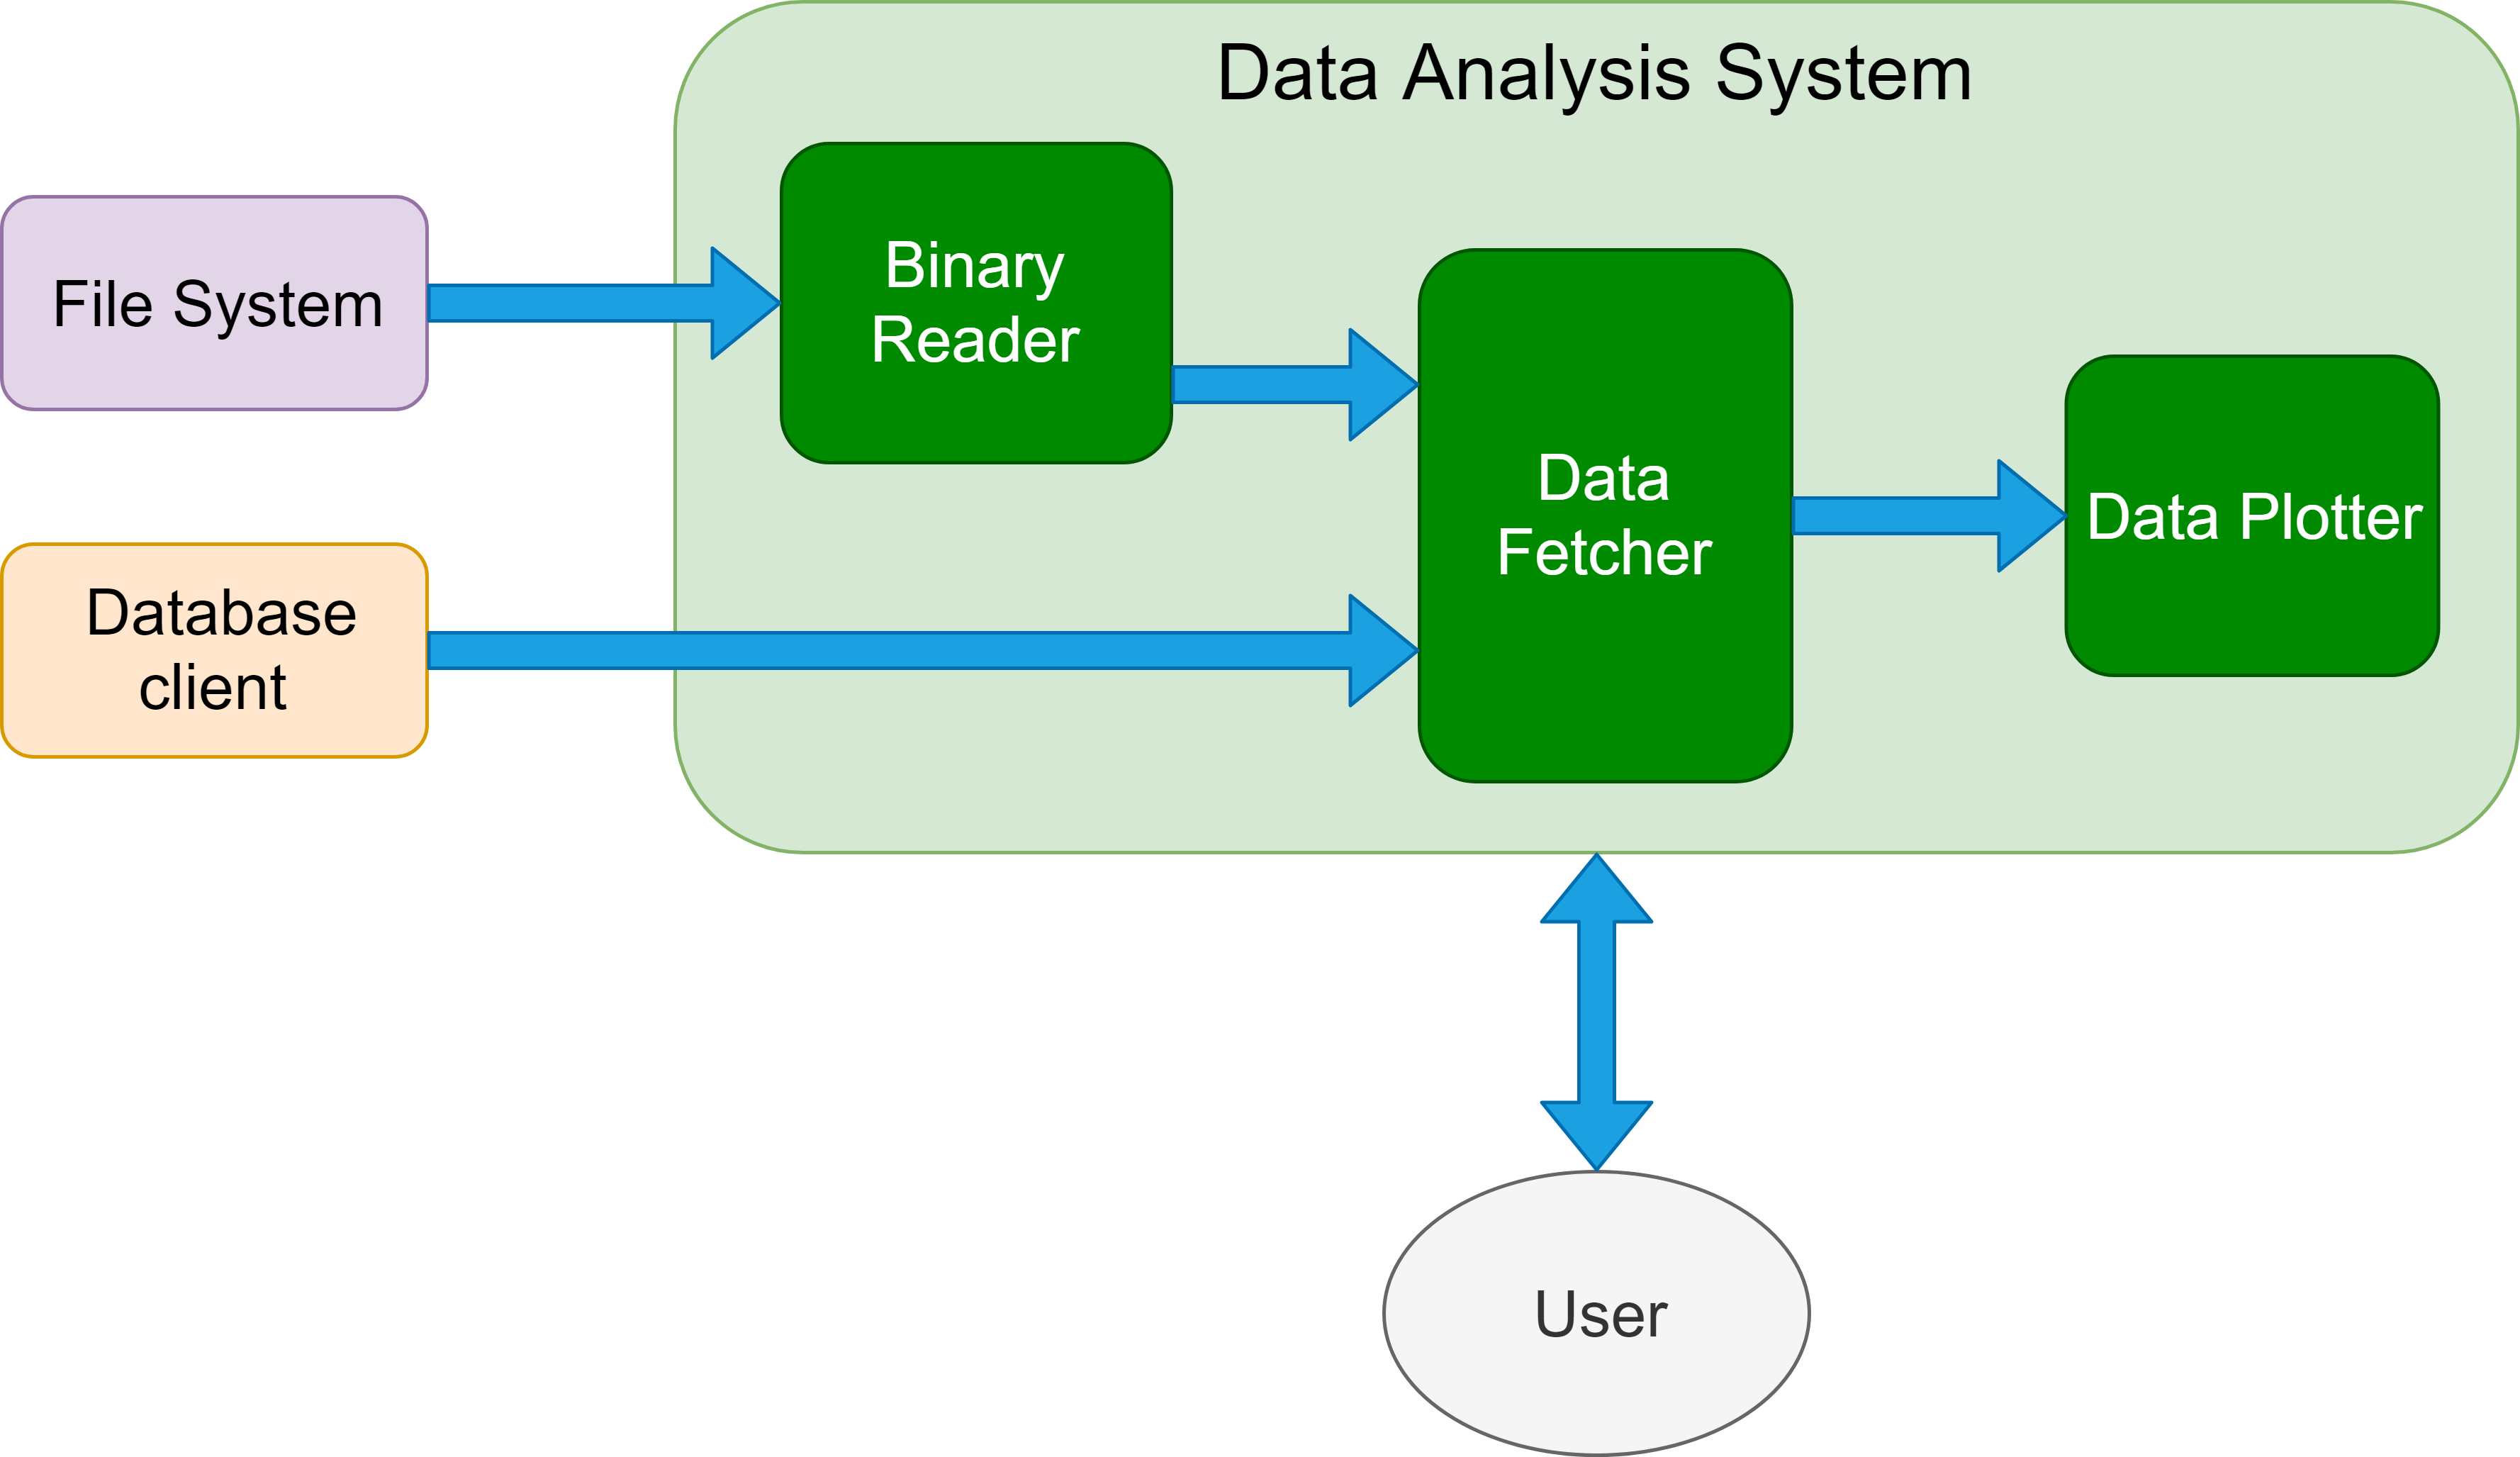
\includegraphics[width=\textwidth]{figures/ArchitetturaDA}
	\caption[Architettura del sistema di analisi dei dati]{ Architettura generale del sistema di analisi dei dati  e le interazioni verso le componenti esterne al sistema stesso.
		\label{fig:ArchitetturaDA}}
\end{figure}


\section{Lettura e contenuto dei file raw}
I file sono creati attraverso LabVIEW\cite{labview}, un programma della National Instruments che si occupa di gestire la lettura dei sensori, e non sono pensati per essere aperti con programmi esterni. Per questo motivo la lettura dei file raw diventa complessa attraverso solo l'uso di Python.

I file raw sono dei file binari che posso essere in uno dei formati proprietari BIN o BIX. Il formato influisce la struttura del file e come sono stati salvati i dati al suo interno.

Il contenuto dei file cambia inoltre in base alla configurazione del Multiphase Flow Meter, di conseguenza ogni BIN e BIX possono essere di tipi diversi, distinti dal campo "BIN type" o "BIX type" all'interno del file.

Ogni file raw contiene un insieme di variabili determinato dal formato e dal tipo del file stesso. Ogni variabile è caratterizzata da:
\begin{itemize}
	\item \texttt{type}: rappresenta il tipo della variabile, ad esempio Int32, UInt32, Float, Boolean.
	\item \texttt{batch size}: rappresenta il numero di letture che vengono effettuate al secondo per quella variabile, può variare da 1 a 2500.
	\item \texttt{data}: un array che contiene le letture effettive del sensore
\end{itemize}

I dati contenuti in queste variabili corrispondo alle letture dei sensori presenti nel Multiphase Flow Meter al momento del test.

\section{Grafici e analisi dei dati}

L'analisi dei dati comincia dalla scelta una delle cartelle dei test presenti nel server aziendale, si ricorda che ogni test rappresenta una serie di letture effettuate in ambiente controllato in un laboratorio. Scelto uno specifico test è possibile creare un grafico di dispersione in base alle proprietà GVF e WLR (descritte nella sezione \ref{"StrutturaDeiDati"}) di tutti i file raw presenti in quella cartella di test. Questa operazione sfrutta le informazioni salvate nel database creato in precedenza in modo da non dover esplorare di nuovo tutta la cartella.
Si ottiene quindi un grafico simile a quello in figura \ref{fig:GVFWLRscatter} dove ogni punto rappresenta un file raw ed è posizionato in base alle proprietà GVF e WLR che aveva il flusso nel momento in cui è stata effettuata la lettura. Si può notare che i punti sono per la maggior parte allineati in una struttura a matrice, questo perché le proprietà del flusso sono variate in modo controllato per coprire più casi possibili. 

\begin{figure}[H]
	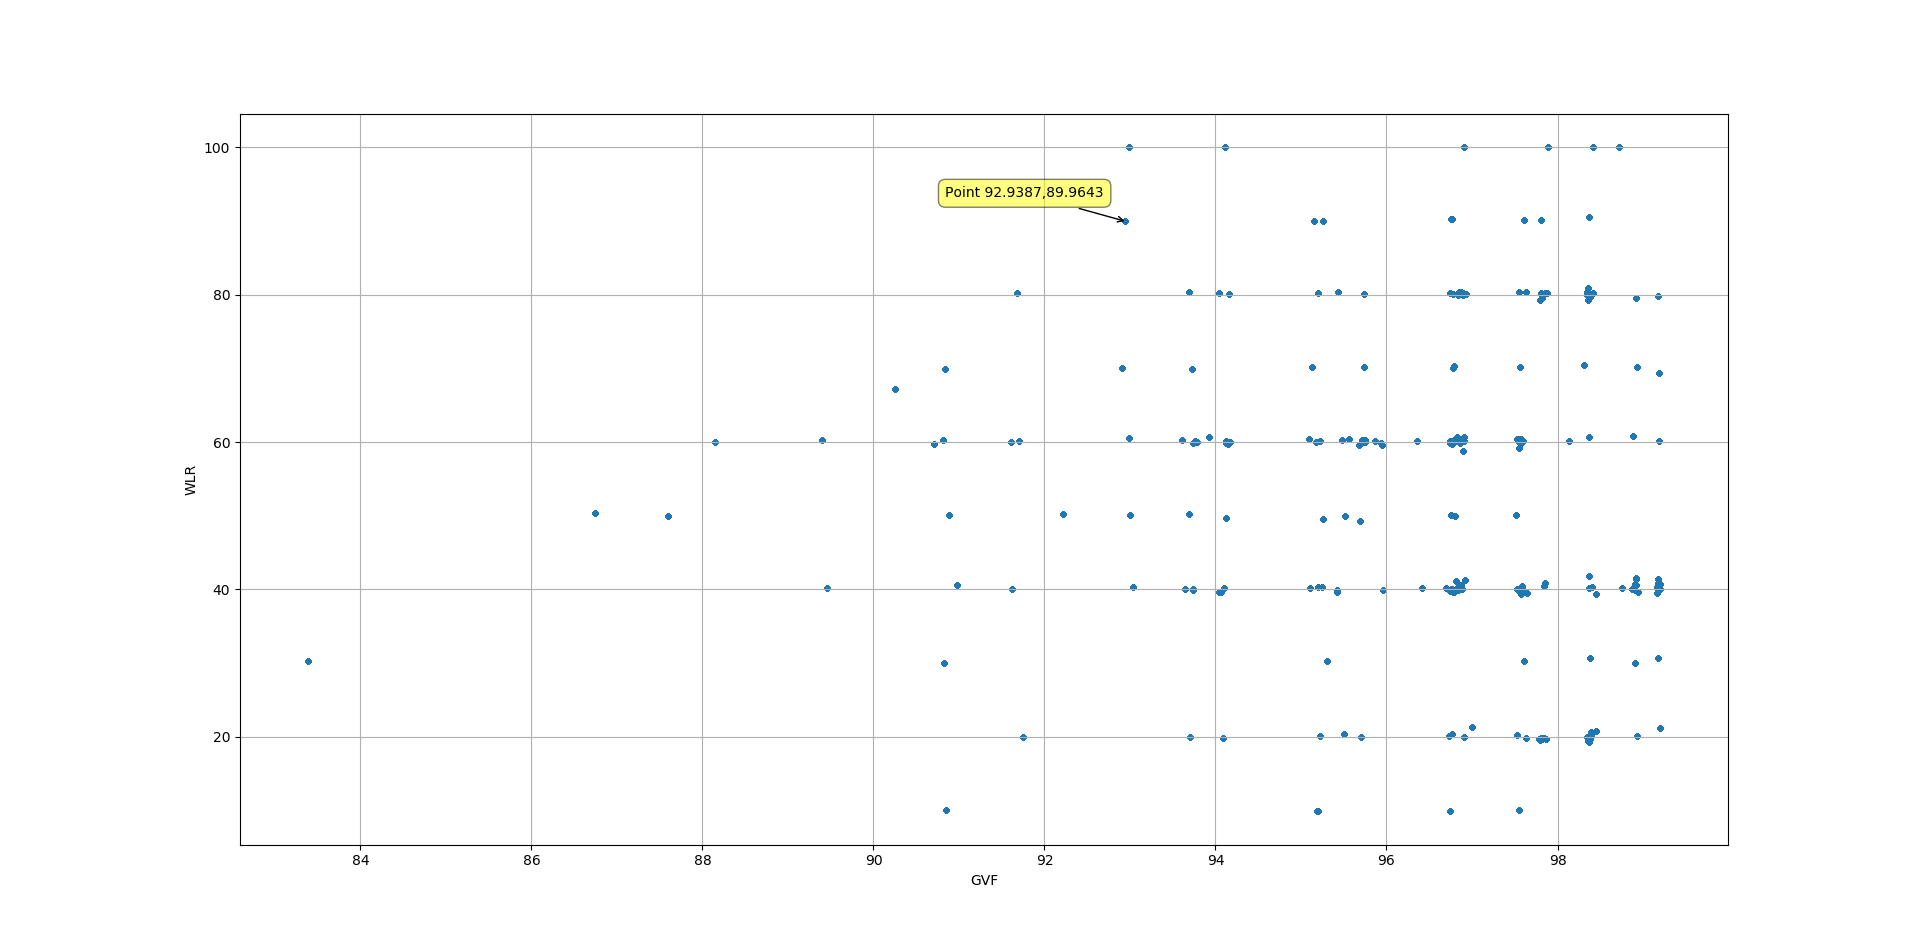
\includegraphics[width=\textwidth]{figures/GVFWLRscatter}
	\caption[Grafico di dispersione GVF-WLR]{ Grafico di dispersione tra le variabili GVF e WLR,  ogni punto rappresenta un file raw ed è posizionato in base alle proprietà GVF e WLR che aveva il flusso nel momento in cui è stata effettuata la lettura. 
		\label{fig:GVFWLRscatter}}
\end{figure}

Cliccando un punto all'interno di questo grafico è possibile vedere graficamente i valori di tutte le variabili del file raw associato a quel punto (figura \ref{fig:MatrixPlot}). Per motivi di velocità e dimensione i grafici delle variabili sono approssimati e contengono solo il massimo in verde, la media in arancione e il minimo in blu di ogni secondo di lettura.

\begin{figure}[H]
	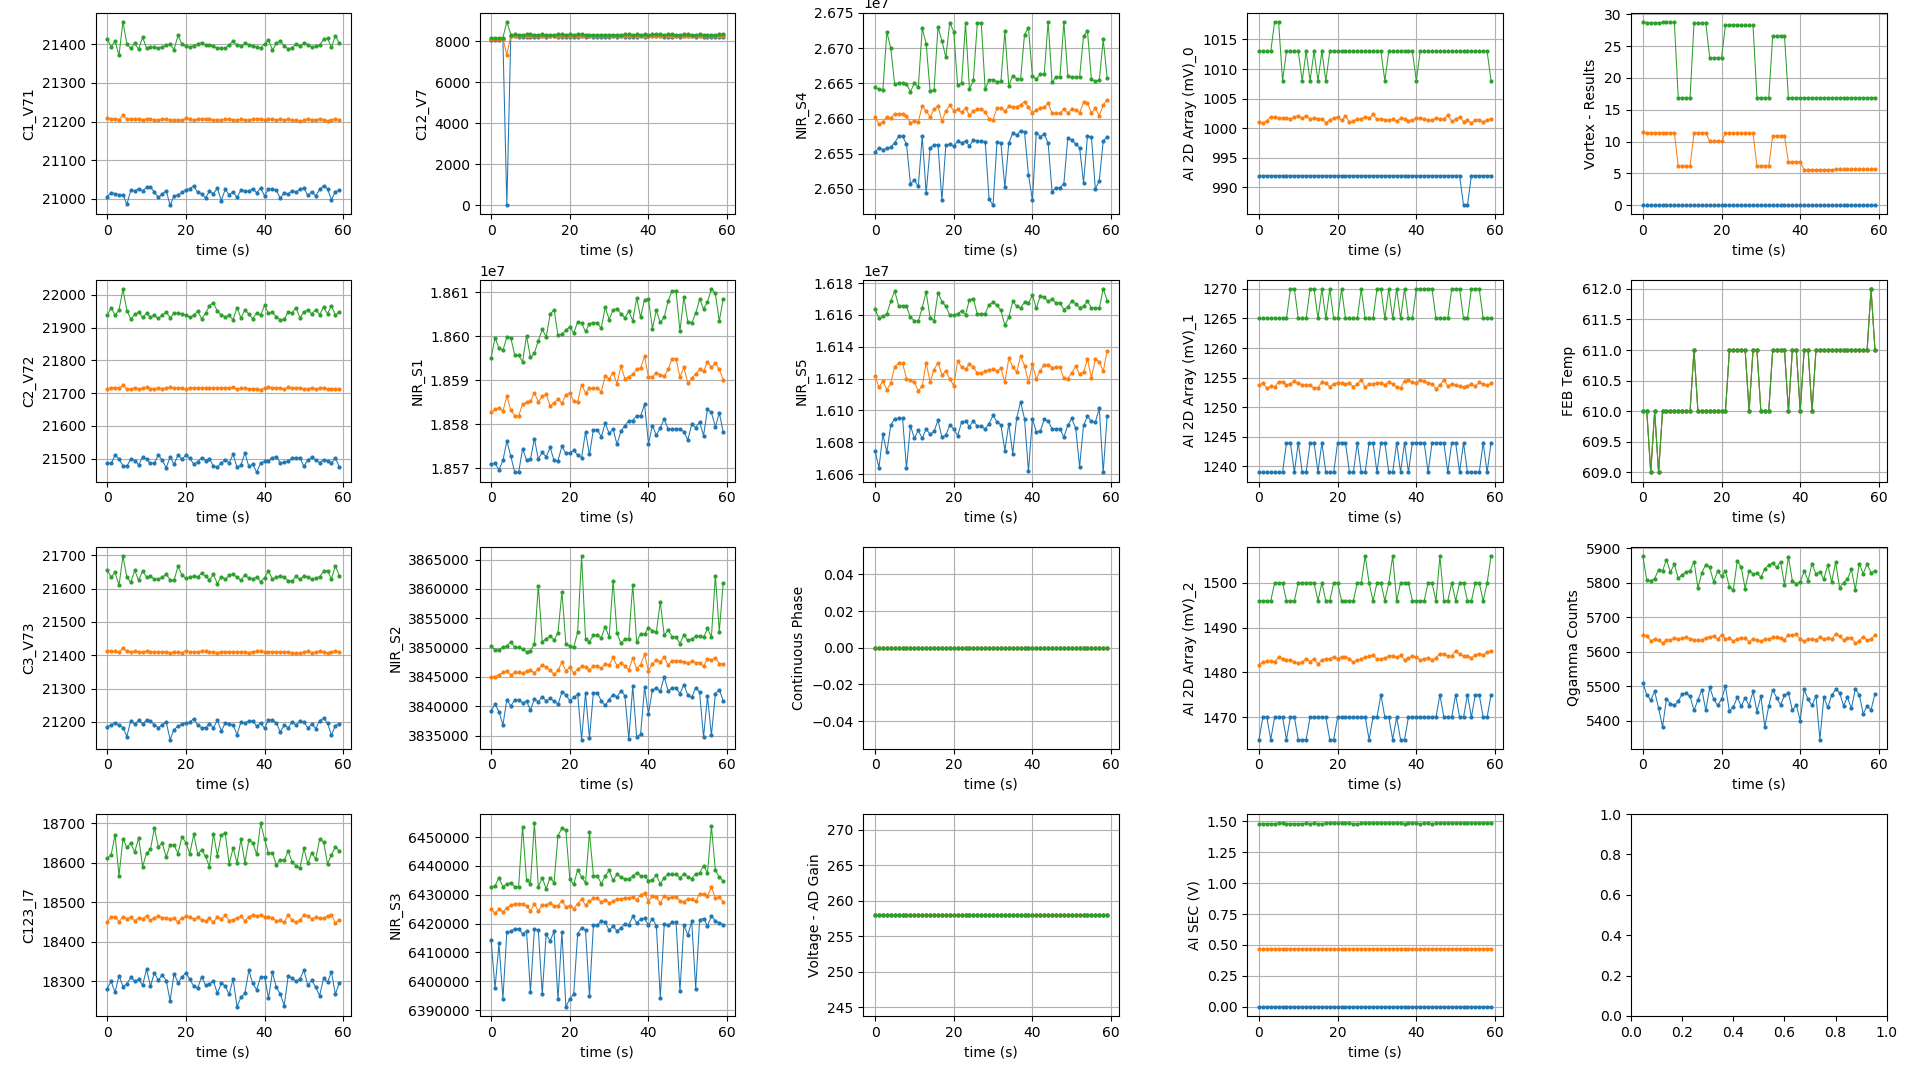
\includegraphics[width=\textwidth]{figures/MatrixPlot}
	\caption[Grafici delle variabili di un file raw]{ Grafici delle variabili di un file raw. La linea in verde indica i massimi di ogni secondo di lettura, in arancione le medie, in blu i minimi.
		\label{fig:MatrixPlot}}
\end{figure}

I grafici delle variabili sono selezionabili tenendo premuto il tasto shift o ctrl della tastiera e cliccando da uno a tre grafici. A seconda del numero di grafici selezionati viene mostrato una tipologia di grafico diversa.

Selezionando un solo grafico si visualizza un nuovo grafico contenente tutti i punti di quella specifica variabile, e non solo un'approssimazione. Allineato al grafico dei punti è presente un istogramma orizzontale che mostra più chiaramente quali sono i valori più frequenti per quella variabile.

\begin{figure}[H]
	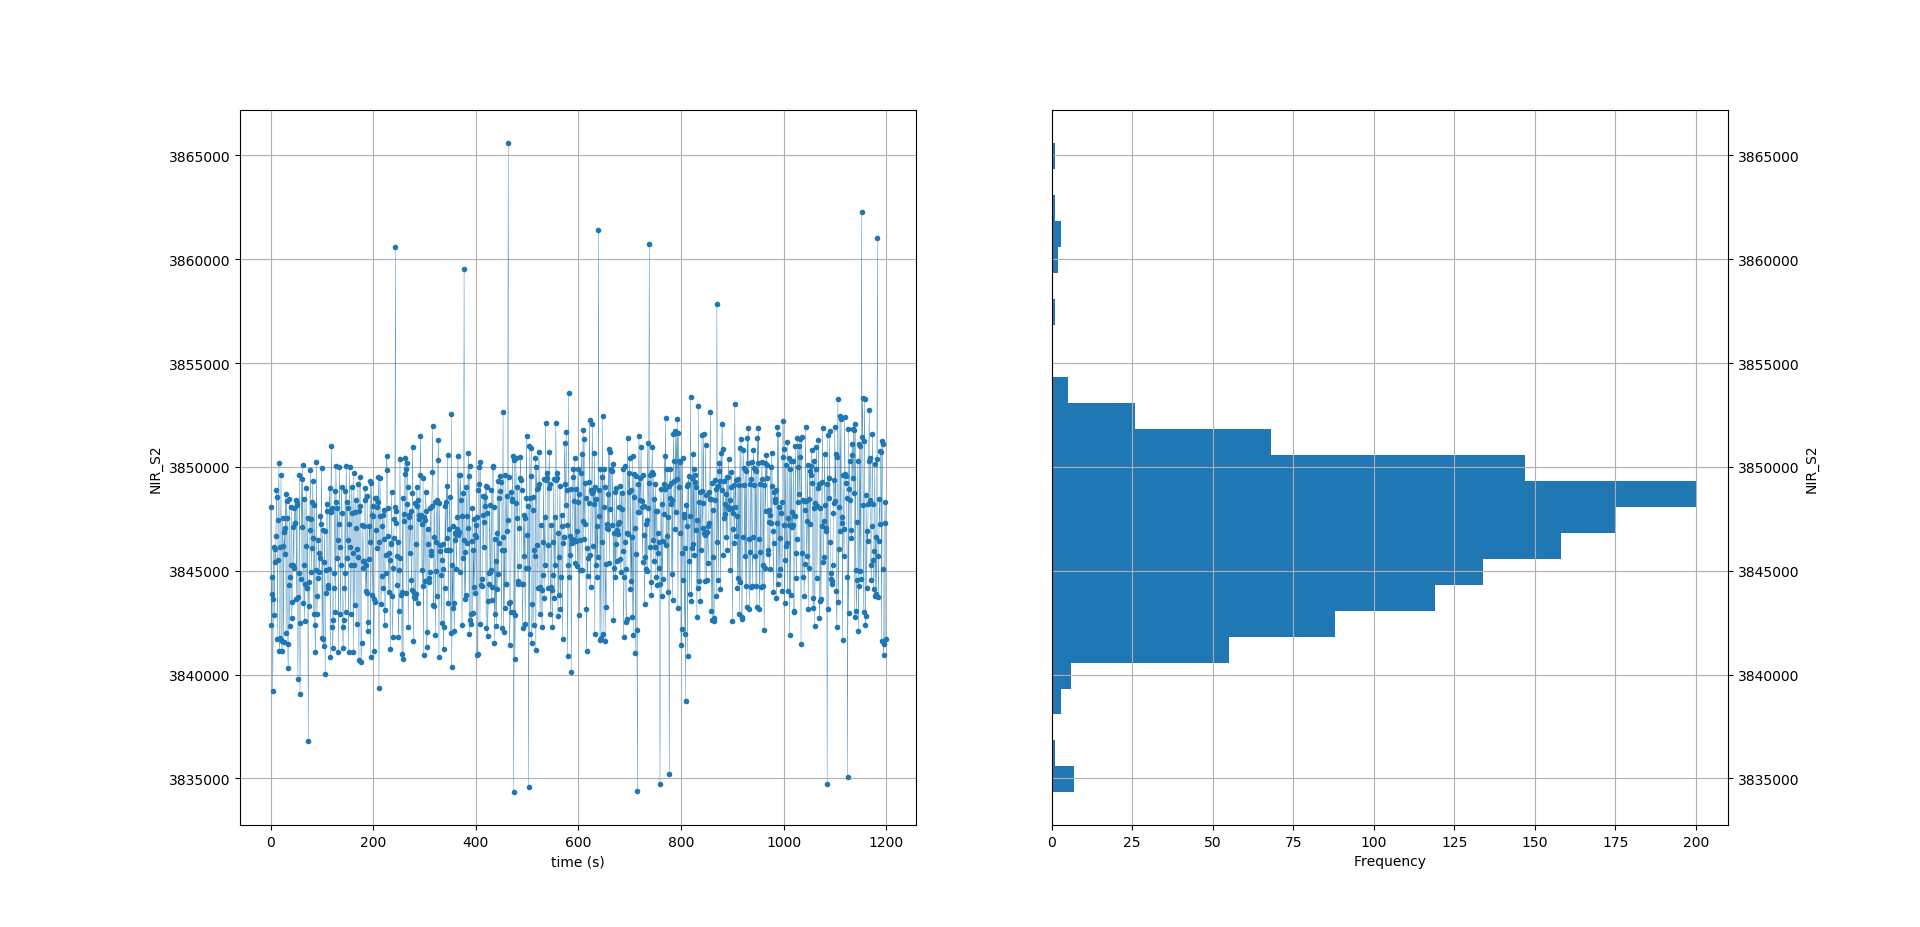
\includegraphics[width=\textwidth]{figures/SimplePlotHistogram}
	\caption[Grafico e istogramma di una variabile]{ Grafico e istogramma di una variabile. L'istogramma rappresenta i valori più frequenti.
		\label{fig:SimplePlotHistogram}}
\end{figure}


Selezionando due grafici si visualizza un grafico di dispersione delle due rispettive variabili. Questo grafico può essere utile per controllare se due variabili sono correlate, punti fuori dalla distribuzione potrebbero indicare delle anomalie. Due variabili correlate si riconoscono dalla posizione dei punti nel grafico stesso, se si dispongono lungo una o più linee diagonali sono correlate, se si dispongono in uno o più gruppi sparsi non sono correlate.

\begin{figure}[H]
	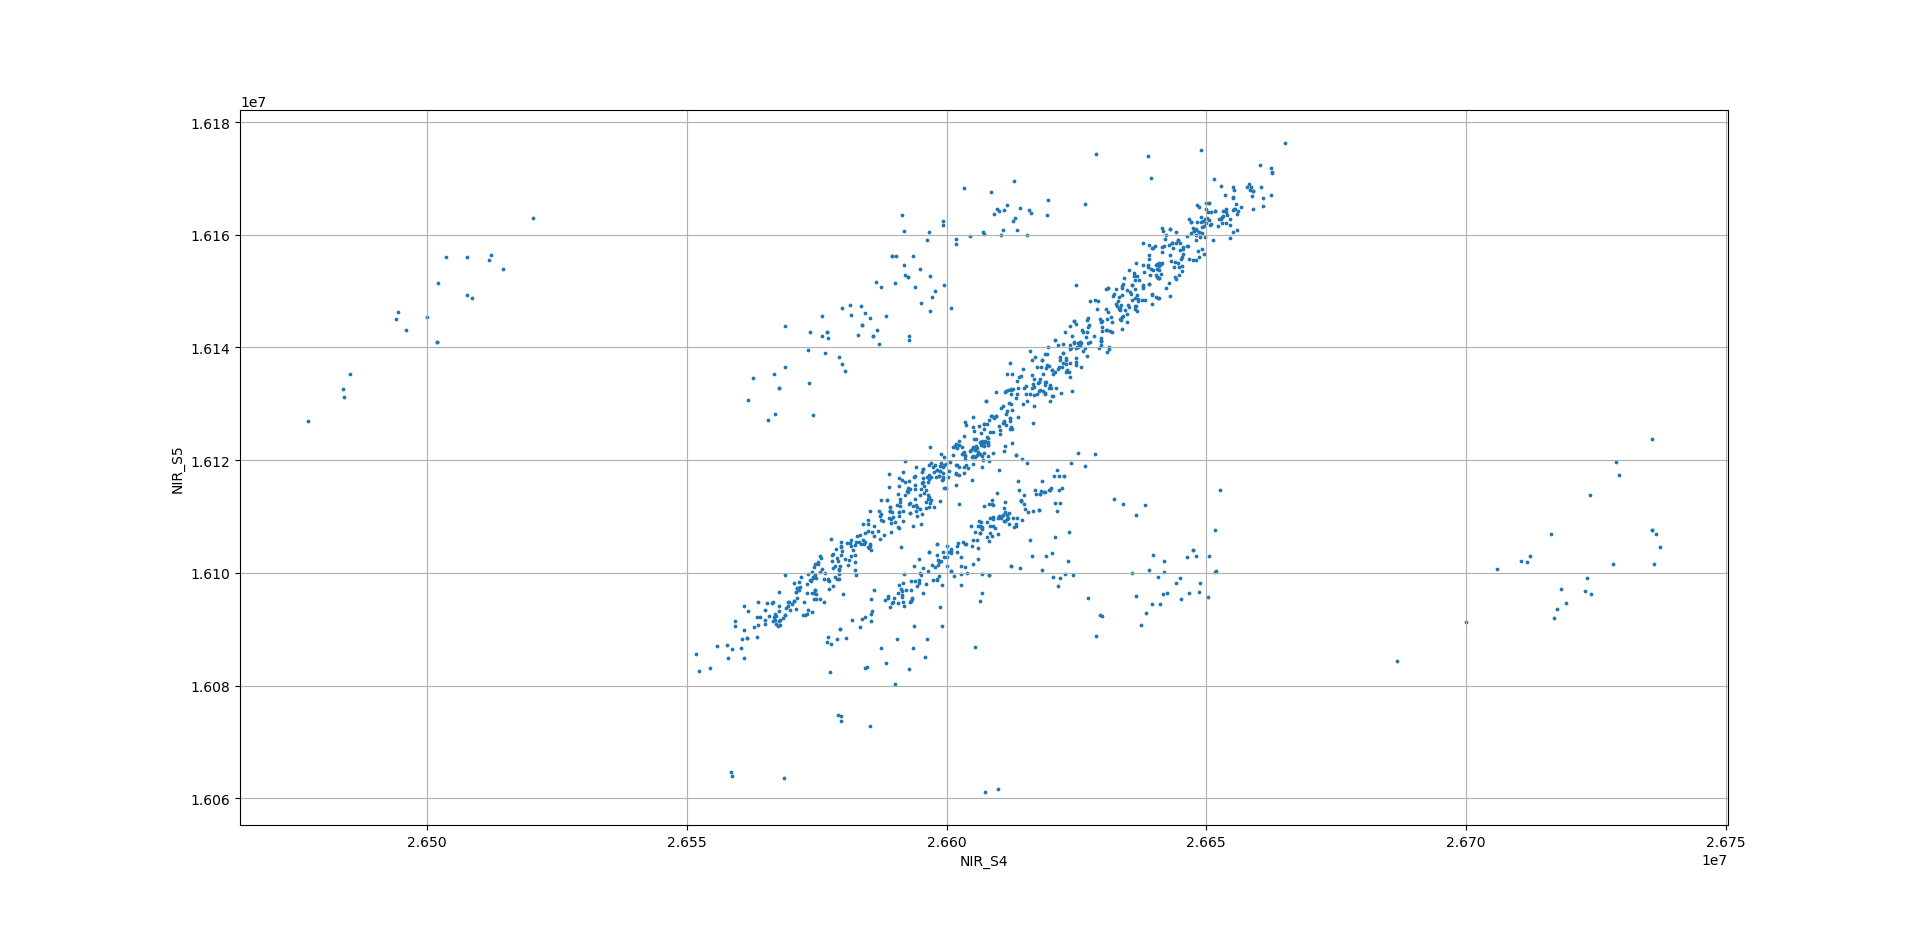
\includegraphics[width=\textwidth]{figures/2Dscatter}
	\caption[Grafico di dispersione di due variabili]{ Grafico di dispersione di due variabili. In questo caso sono si può notare che sono correlate.
		\label{fig:2Dscatter}}
\end{figure}

Selezionando tre grafici si visualizza un grafico di dispersione in 3D delle tre variabili selezionate, che si può spostare e ruotare a piacimento. Questo grafico è particolarmente utile quando si utilizzano tre variabili correlate tra di loro.

\begin{figure}[H]
	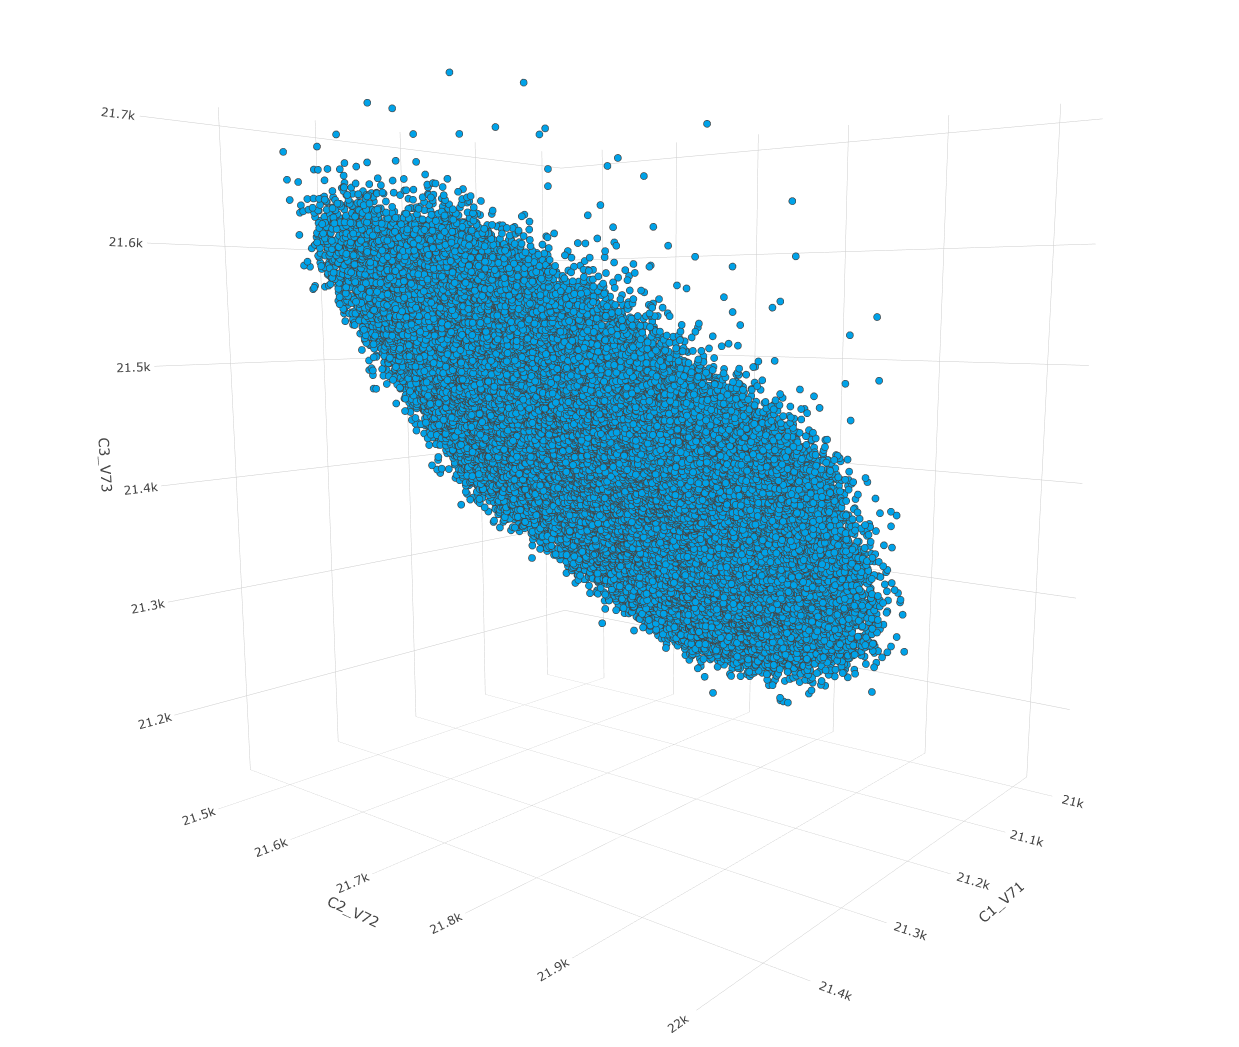
\includegraphics[width=\textwidth]{figures/3Dscatter}
	\caption[Grafico di dispersione di tre variabili]{ Grafico di dispersione di tre variabili. In questo caso i punti sono disposti a forma di disco perché le variabili C1\_V71 e C3\_V73 sono correlate tra loro ma non a C2\_V72.
		\label{fig:3Dscatter}}
\end{figure}

Ogni tipologia di grafico può essere visualizzata usando la libreria matplotlib\cite{matplotlib} oppure plotly\cite{plotly} in base a se si sono selezionai i grafici con shift o con ctrl. Si è lasciata la scelta perché entrambe le librerie hanno dei vantaggi e degli svantaggi a seconda del grafico che si vuole ottenere.

matplotlib è molto veloce nella creazione del grafico ma con molti punti, intorno alle decine di migliaia, rallenta quando si prova a ingrandire, ruotare e selezionare una parte specifica del grafico.
plotly impiega un paio di minuti per la creazione del grafico perché genera una pagina HTML indipendente, ma la manipolazione del grafico risulta veloce anche nell'ordine delle centinaia di migliaia di punti. Inoltre, essendo i grafici file HTML veri e propri, possono essere salvati e visualizzati offline, mentre matplotlib permette solo il salvataggio di un'immagine statica del grafico perdendo l'interattività.


%!TEX root = ../dissertation.tex
\chapter{Autodiagnostica di anomalie}
\label{AutodiagnosticaDiAnomalie}

Questo capitolo tratta l'addestramento di vari algoritmi di machine learning e la valutazione di essi, tratta inoltre il processo di feature extraction applicato ai dati prima di essere utilizzati.

\section{Feature extraction}
Nell'ambito del machine learning con feature extraction si intende l'estrazione di caratteristiche dai dati di ingresso per semplificare in seguito l'apprendimento.
L'estrazione di feature è particolarmente utile quando il numero di dati in ingresso all'algoritmo di machine learning è molto alto, e renderebbe l'apprendimento troppo lungo e complesso \cite{FeatureExtraction}.

Nel caso del Multiphase Flow Meter alcuni dei sensori effettuano fino a 2500 letture al secondo, e in un solo minuto di registrazione si ottengono già 150000 valori per uno solo delle 20 o 30 variabili lette dai sensori presenti nel MPFM.
Per questo motivo prima di allenare un algoritmo di machine learning bisogna estrarre alcune feature da questi dati.

\subsection{tsfresh}
tsfresh è la libreria utilizzata per l'estrazione di feature in quanto specifica per le serie temporali, ovvero serie dove i dati sono legati all'istante di tempo in qui sono stati osservati, come per le letture dei sensori del MPFM \cite{tsfresh}.

tsfresh permette quindi di calcolare automaticamente un certo numero di feature su una serie temporale qualsiasi. Sono presenti più di 100 feature estraibili con tsfresh ma estrarle tutte richiederebbe troppo tempo e spesso risultano ridondanti in questo contesto.

\begin{figure}
	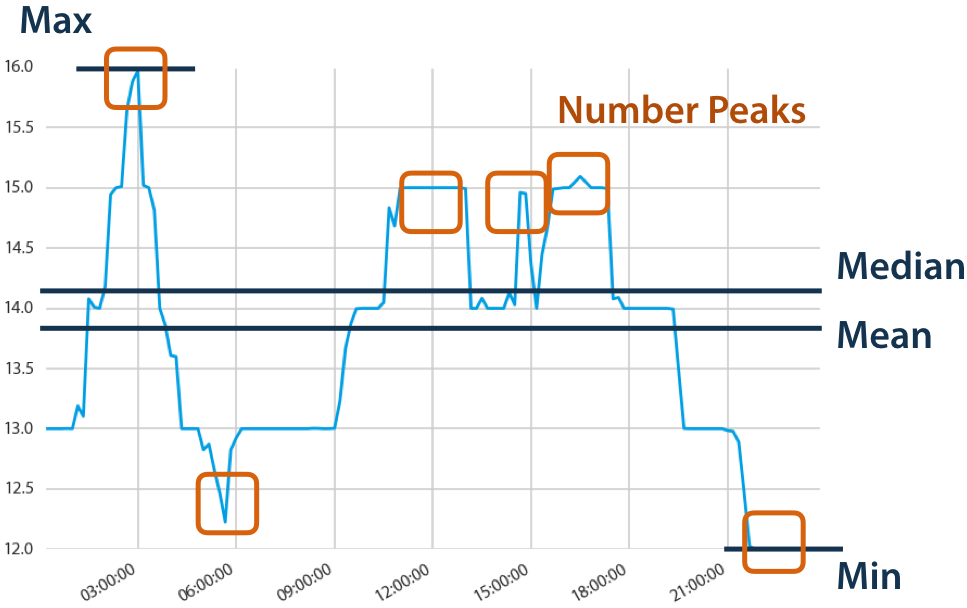
\includegraphics[width=\textwidth]{figures/tsfresh_features}
	\caption[Esempio di features estratte dalla libreria tsfresh]{ Esempio di alcune features estraibili da una serie temporale attraverso la libreria tsfresh
		
		\label{fig:tsfresh_features}}
\end{figure}

Si è scelto quindi un set ridotto di feature che comprende solamente il minimo, massimo, media, mediana, deviazione standard e varianza di ogni minuto di dati per ogni sensore. In questo modo il tempo di estrazione si riduce drasticamente, ma rimane comunque notevole quando lo si deve applicare a più file raw per avere un insieme di dati sufficiente per l'apprendimento.

Per non ripetere l'estrazione di feature ogni volta che si vuole applicare un algoritmo di machine learning, è stata effettuata l'estrazione delle feature di tutte le variabili di tutti i file raw una volta sola e il risultato è stato salvato in una tabella apposita nel database. Questo processo ha richiesto circa 8 ore per il completamento, ma una volta presenti nel database le feature si possono ottenere istantaneamente.

\section{Anomaly detection}

L'anomaly detection consiste nella identificazione di osservazioni o eventi che differiscono sostanzialmente dalla maggior parte degli altri dati. Nel contesto del Multiphase Flow meter queste anomalie nei dati possono corrispondere a dei problemi o difetti nello strumento o nei sensori stessi. Per questo motivo individuare le anomalie attraverso algoritmi di machine learning può essere utile per diagnosticare lo stato dello strumento, e in alcuni casi prevedere quando si sta per rompere prima che accada.

Esistono due tecniche principali di anomaly detection. L'anomaly detection supervisionato richiede che i dati siano classificati come "normali" oppure "anormali" e sfrutta questa proprietà per classificare i nuovi dati dopo l'apprendimento. L'anomaly detection non supervisionato non richiede nessuna classificazione dei dati e assume che la maggior parte dei dati siano normali e cerca i punti  meno simili agli altri \cite{AnomalyDetection}.

Le letture effettuate dei sensori durante i test non sono classificate quindi è necessario usare un approccio non supervisionato. 

\subsection{scikit-learn e PyOD}
scikit-learn è una libreria che offre una vasta quantità di strumenti e funzioni per machine learning in Python, tra i quali implementazioni degli algoritmi più comuni, metodi per estrarre feature e normalizzare i dati e molto altro \cite{scikit-learn}.
PyOD invece è una libreria più semplice, specifica per lavorare nel campo dell'anomaly detection e spesso sfrutta alcune delle funzionalità offerte da scikit-learn \cite{zhao2019pyod}.

Da queste librerie sono stati scelti 5 degli algoritmi più utilizzati per l'anomaly detection e sono stati valutati e confrontati tra loro.

\subsection{Histogram-Based Outlier Detection (HBOS)}
In questo algoritmo viene costruito un istogramma per ogni variabile e la combinazione di tutti gli istogrammi viene utilizzata per determinare quali punti sono "outlier" ovvero anomalie. Questo algoritmo assume che i data normali siano concentrati in una particolare zona e non performa altrettanto bene se i dati sono divisi in diversi cluster. In compenso è uno degli algoritmi più efficienti e classifica i dati in tempo lineare O(n) oppure O(n*log(n)) a seconda se il "bin size" è statico o dinamico \cite{HBOS}.

\subsection{Isolation Forest}
Isolation Forest è un algoritmo che si concentra su isolare le anomalie che sono definite come i punti più rari e isolati. In breve una foresta di alberi binari di ricerca è costruita seguendo un approccio che divide casualmente in due lo spazio dei punti. Ad ogni iterazione ogni parte è divisa a sua volta in due fino a quando contiene un solo punto. I punti più isolati saranno separati dagli altri in un minor numero di tagli e saranno quindi più vicini alla radice dell'albero binario. A tutti i punti viene quindi assegnato un punteggio in base alla loro altezza nell'albero, dove le anomalie avranno punteggio più alto in quanto sono più vicine alla radice e i punti normali un punteggio più basso in quanto più distanti dalla radice \cite{IF}.


\subsection{K-Nearest Neighbors (KNN)}
Questo algoritmo si basa sulla distanza di ogni punto dai suoi k punti più vicini per determinare gli "inlier" e gli "outlier" ovvero i punti normali e le anomalie. La distanza di un punto dai suoi vicini è usata quindi per dare un punteggio di quanto anomalo è il punto stesso \cite{KNN}.	

\subsection{Local Outlier Factor (LOF)}
Local Outlier Factor è un algoritmo basato sul confronto tra la densità di un punto e la densità dei suoi punti più vicini. Considera quindi come outlier i punti che hanno minor densità rispetto ai loro punti più vicini. La località dell'algoritmo permette di riconoscere anomalie che non sarebbero considerate da altri algoritmi, ma questo approccio spesso è applicabile solo a spazi di dati con poche dimensioni \cite{LOF}.

\subsection{Principal Component Analysis (PCA)}
A differenza dell'Isolation Forest questo metodo cerca di classificare gli "inlier" e considera i punti rimanenti come anomalie. Spesso è utilizzato quando si lavora con spazi di dati a molte dimensioni, oppure quando il numero di anomalie è basso e classificarle risulta più difficile di classificare i punti normali. PCA determina quale caratterista ha il maggior impatto sulla varianza dei dati, ovvero determina le componenti principali \cite{PCA}.

\subsection{Addestramento e confronto} \label{AddestramentoEConfronto}

Per l'addestramento degli algoritmi sono state utilizzate le feature estratte in precedenza e caricate nel database. In particolare queste feature sono: massimo, minimo, media, mediana, varianza, deviazione standard di un minuto di dati. Ogni confronto è stato ripetuto per 3 variabili differenti, in particolare sono state utilizzate C1\_V71\_0 che misura la capacità del fluido, C1\_V71\_1 che misura la resistenza del fluido, e NIR\_S1 che è uno dei sensori che misura il WLR.
Per la variabile C1\_V71\_0 sono stati utilizzati 5369 minuti di dati, questo numero corrisponde quindi al numero di sample usato nell'apprendimento. Per la variabile C1\_V71\_1 invece sono stati utilizzati 1122 sample, e infine per NIR\_S1 7267 sample.
La dimensione dei dati dipende dal numero di feature utilizzate, in questo caso è 6 per tutte e tre le variabili.

Non conoscendo quali dei punti sono veramente anomalie, o se i dati non contengono nessuna anomalia, si è deciso di aggiungere del rumore casuale entro il minimo e il massimo dei punti. I punti che formano il rumore possono essere quindi considerati come le anomalie da trovare. 

Di conseguenza ad ogni variabile è stato aggiunto un numero di punti casuale pari al 10\% del numero di sample iniziale. La valutazione di un algoritmo dipende dal numero di punti aggiunti casualmente classificati correttamente come outlier, e dal numero di punti originali classificati correttamente come inlier.

\begin{figure} [H]
	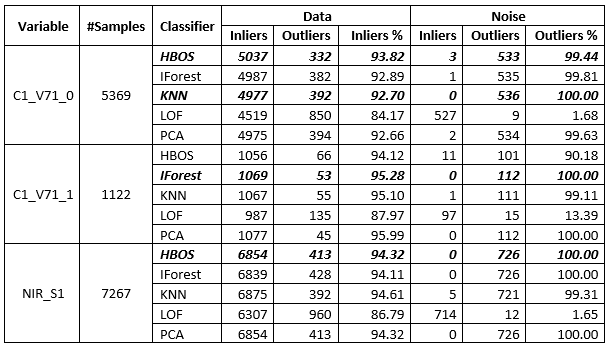
\includegraphics[width=\textwidth]{figures/homogeneous_noise}
	%\caption[Esempio di features estratte dalla libreria tsfresh]{
		
	%\label{fig:homogeneous_noise}}
\end{figure}

Dai risultati si può vedere come tutti gli algoritmi siano riusciti a classificare correttamente come outlier praticamente tutto il rumore, tranne per LOF che non ha riconosciuto il rumore come anomalia in nessuna delle tre variabili.

Infine l'addestramento è stato ripetuto con l'aggiunta di rumore non più omogeneamente, ma raggruppato in 5 cluster casuali.

\begin{figure} [H]
	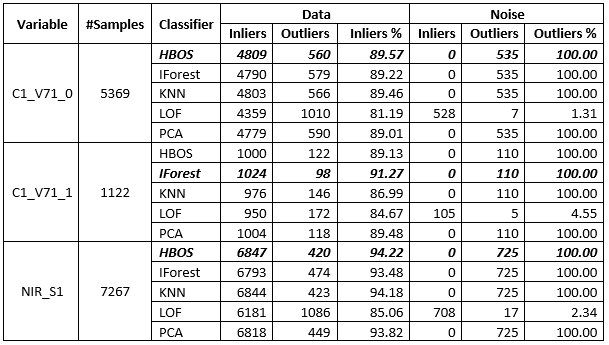
\includegraphics[width=\textwidth]{figures/cluster_noise}
	%\caption[Esempio di features estratte dalla libreria tsfresh]{
	
	%\label{fig:homogeneous_noise}}
\end{figure}

In questo caso tutti gli algoritmi hanno performato addirittura meglio, probabilmente perché il cluster erano troppo distanti dalla maggior parte dei dati e troppo poco densi per confondere gli algoritmi basati sulla densità. LOF non riesce ancora a distinguere correttamente il rumore, forse per una configurazione sbagliata nel momento dell'apprendimento.

\section{Visualizzazione delle anomalie}

Per verificare il funzionamento degli algoritmi, e avere un'idea sulla motivazione delle scelte effettuate dagli algoritmi nel momento della classificazione, sono stati creati dei grafici che mostrano i dati iniziali e la loro classificazione dopo l'addestramento.

Nei seguenti grafici è stato utilizzato l'algoritmo HBOS addestrato sulla variabile C1\_V71\_0. L'addestramento comprende tutte e 6 le feature utilizzate in precedenza, ma per poter creare un grafico in due dimensioni sono state utilizzate la deviazione standard nelle ascisse e la media nelle ordinate.

\subsection{Visualizzazione degli outlier}
Nel grafico in figura \ref{fig:vis1} i punti in rosso sono stati classificati come outlier, mentre quelli in verde come inlier. Anche se a prima vista il numero di outlier sembra molto maggiore degli inlier, dall'istogramma si può vedere che è esattamente il contrario. La maggior parte dei punti è altamente concentrata in una piccola zona, i punti lontani da questa concentrazione sono stati quindi classificati come anomalie.

\begin{figure} [H]
	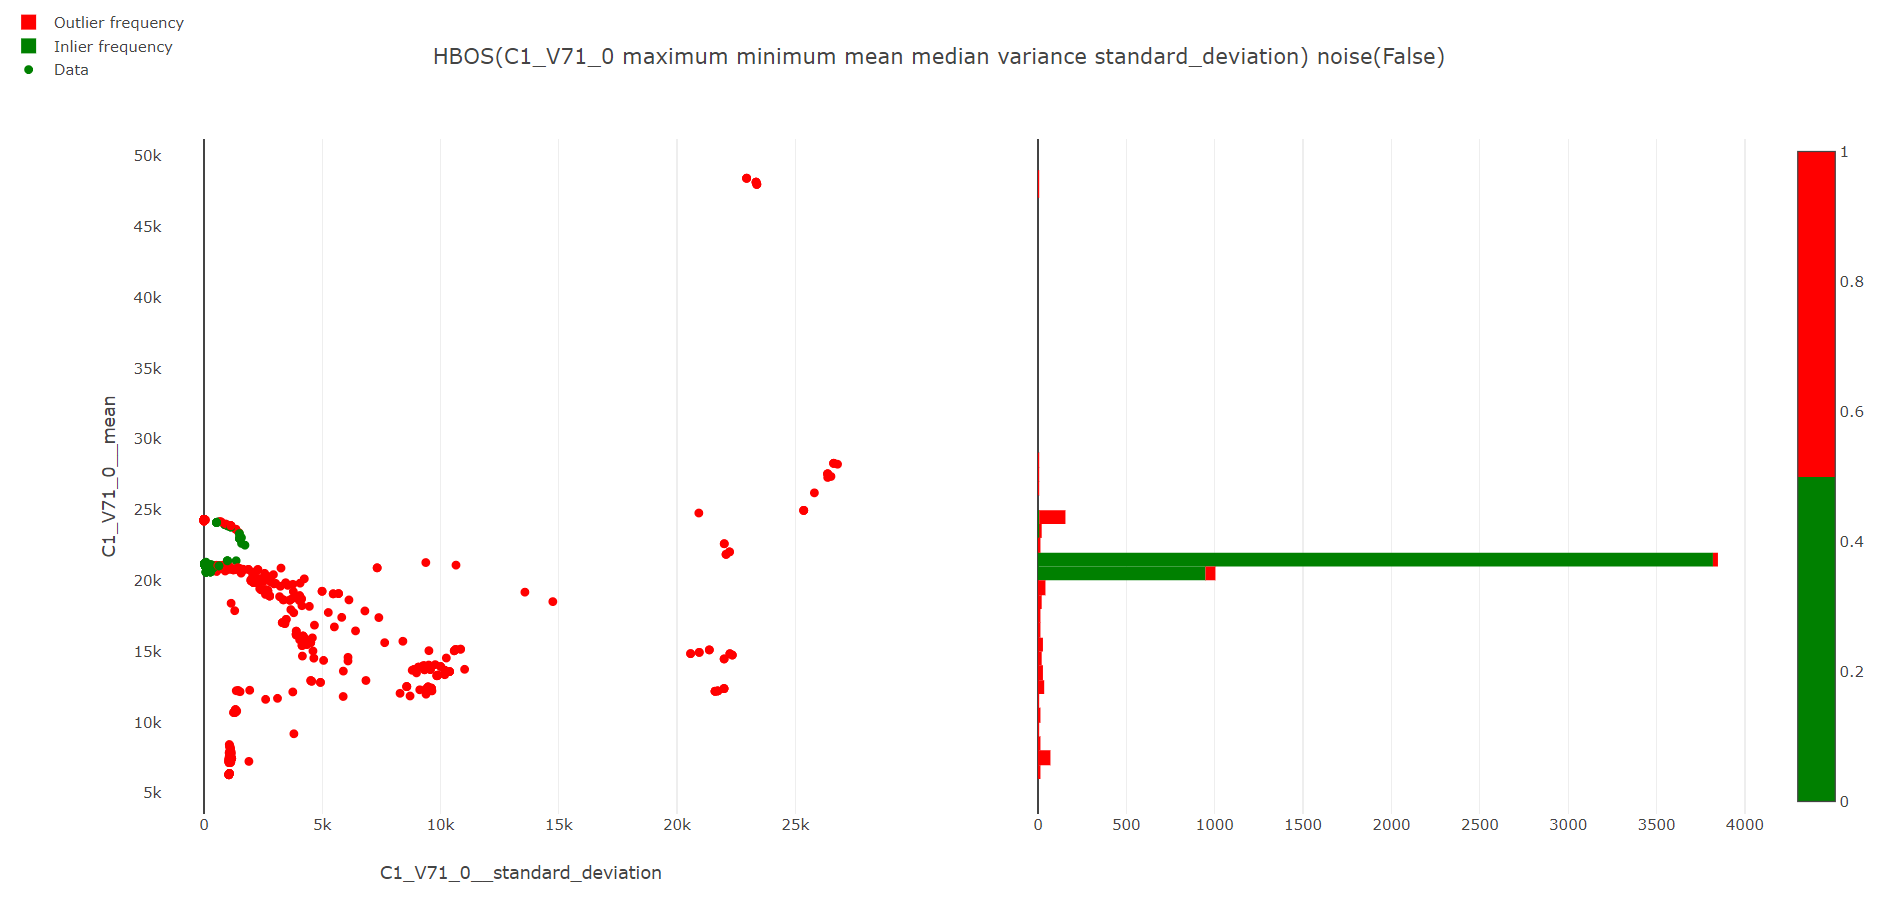
\includegraphics[width=\textwidth]{figures/vis1}
	\caption[Grafico dell'anomaly detection nella variabile C1\_V71\_0 con HBOS]{Grafico dell'anomaly detection nella variabile C1\_V71\_0 con HBOS. In rosso gli outlier, in verde gli inlier.
	
	\label{fig:vis1}}
\end{figure}

\subsection{Visualizzazione dello score dei punti}
A ogni punto viene assegnato uno punteggio o score in base dall'algoritmo utilizzato, questo punteggio è un valore da 0 a 1 che determina quanto sicuro è l'algoritmo nella classificazione del punto. In figura \ref{fig:vis2} si può vedere lo score di ogni punto in base al colore, i punti vicino al giallo sono più probabilmente outlier mentre i punti vicino al blu scuro sono più probabilmente inlier. In questo caso il colore dell'istogramma è irrilevante.

\begin{figure} [H]
	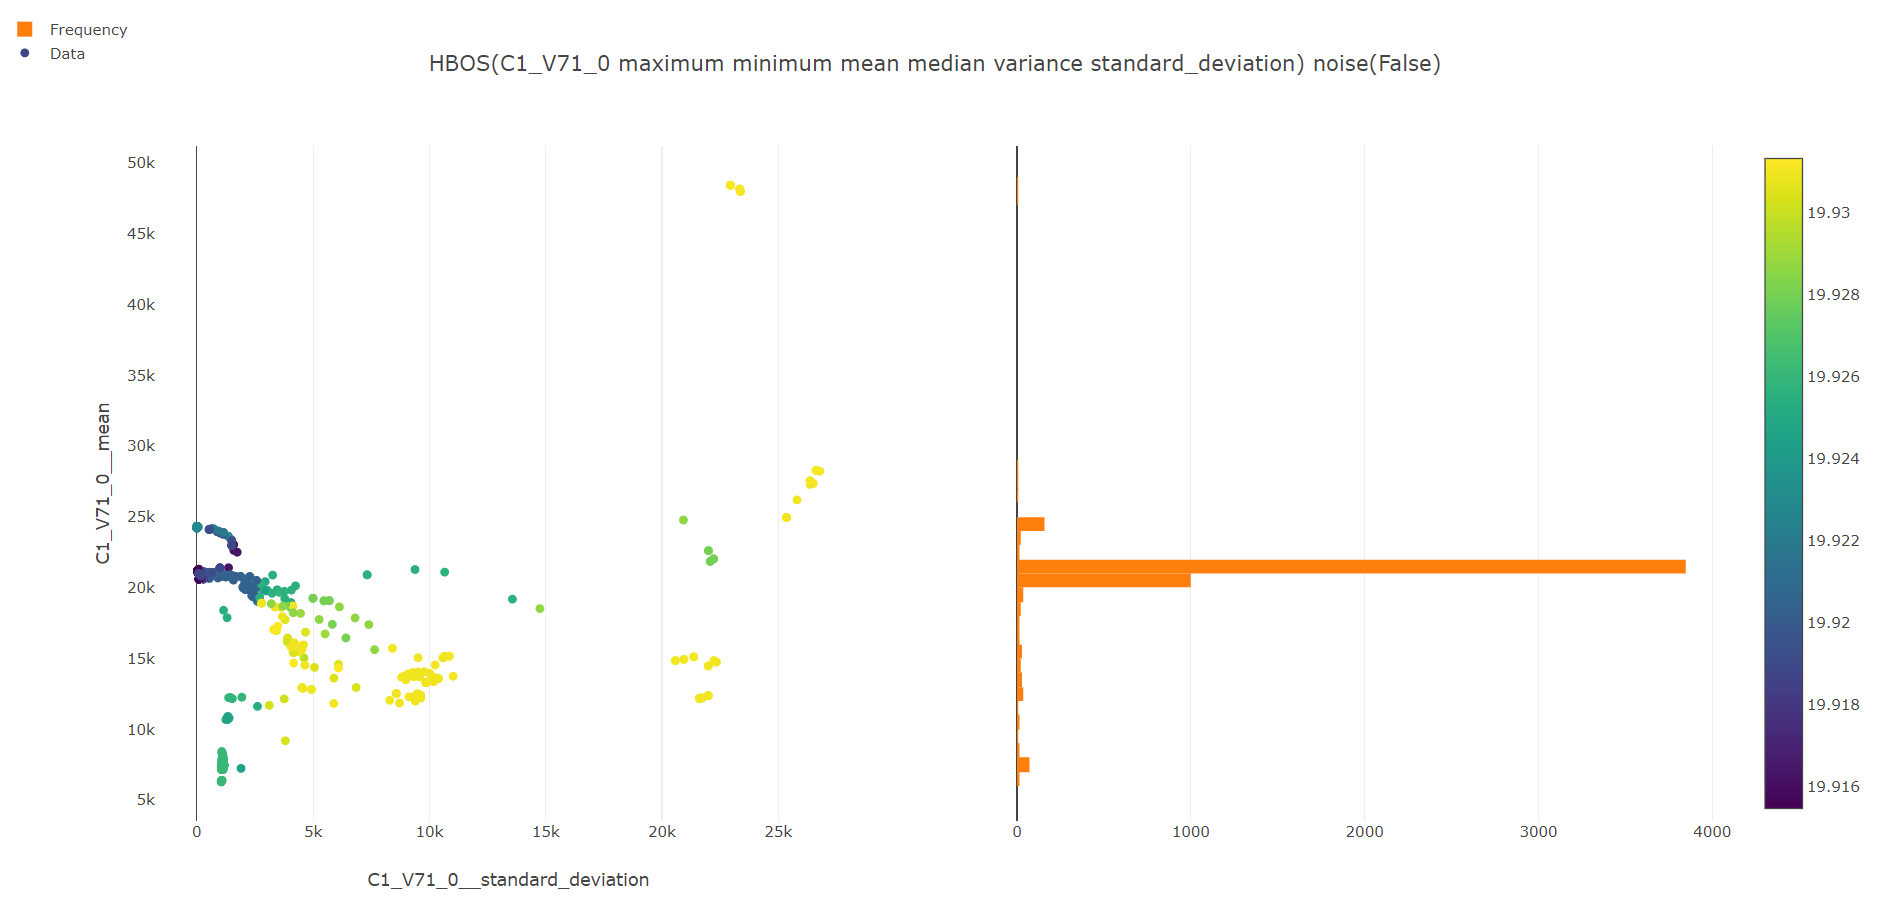
\includegraphics[width=\textwidth]{figures/vis2}
	\caption[Grafico dello score dei punti usando HBOS e la variabile C1\_V71\_0]{Grafico dello score dei punti usando HBOS e la variabile C1\_V71\_0. I punti verso il giallo sono più probabilmente outlier, mentre i punti verso il blu scuro sono più probabilmente inlier.
		
		\label{fig:vis2}}
\end{figure}

\subsection{Visualizzazione dello score con rumore omogeneo}
Nel grafico in figura \ref{fig:vis3} è stato aggiunto casualmente del rumore pari al 10\% dei punti iniziali. I dati iniziali sono rappresentati con dei pallini mentre il rumore con dei triangoli, tutti i punti sono colorati in base allo score assegnato dall'algoritmo.

\begin{figure} [H]
	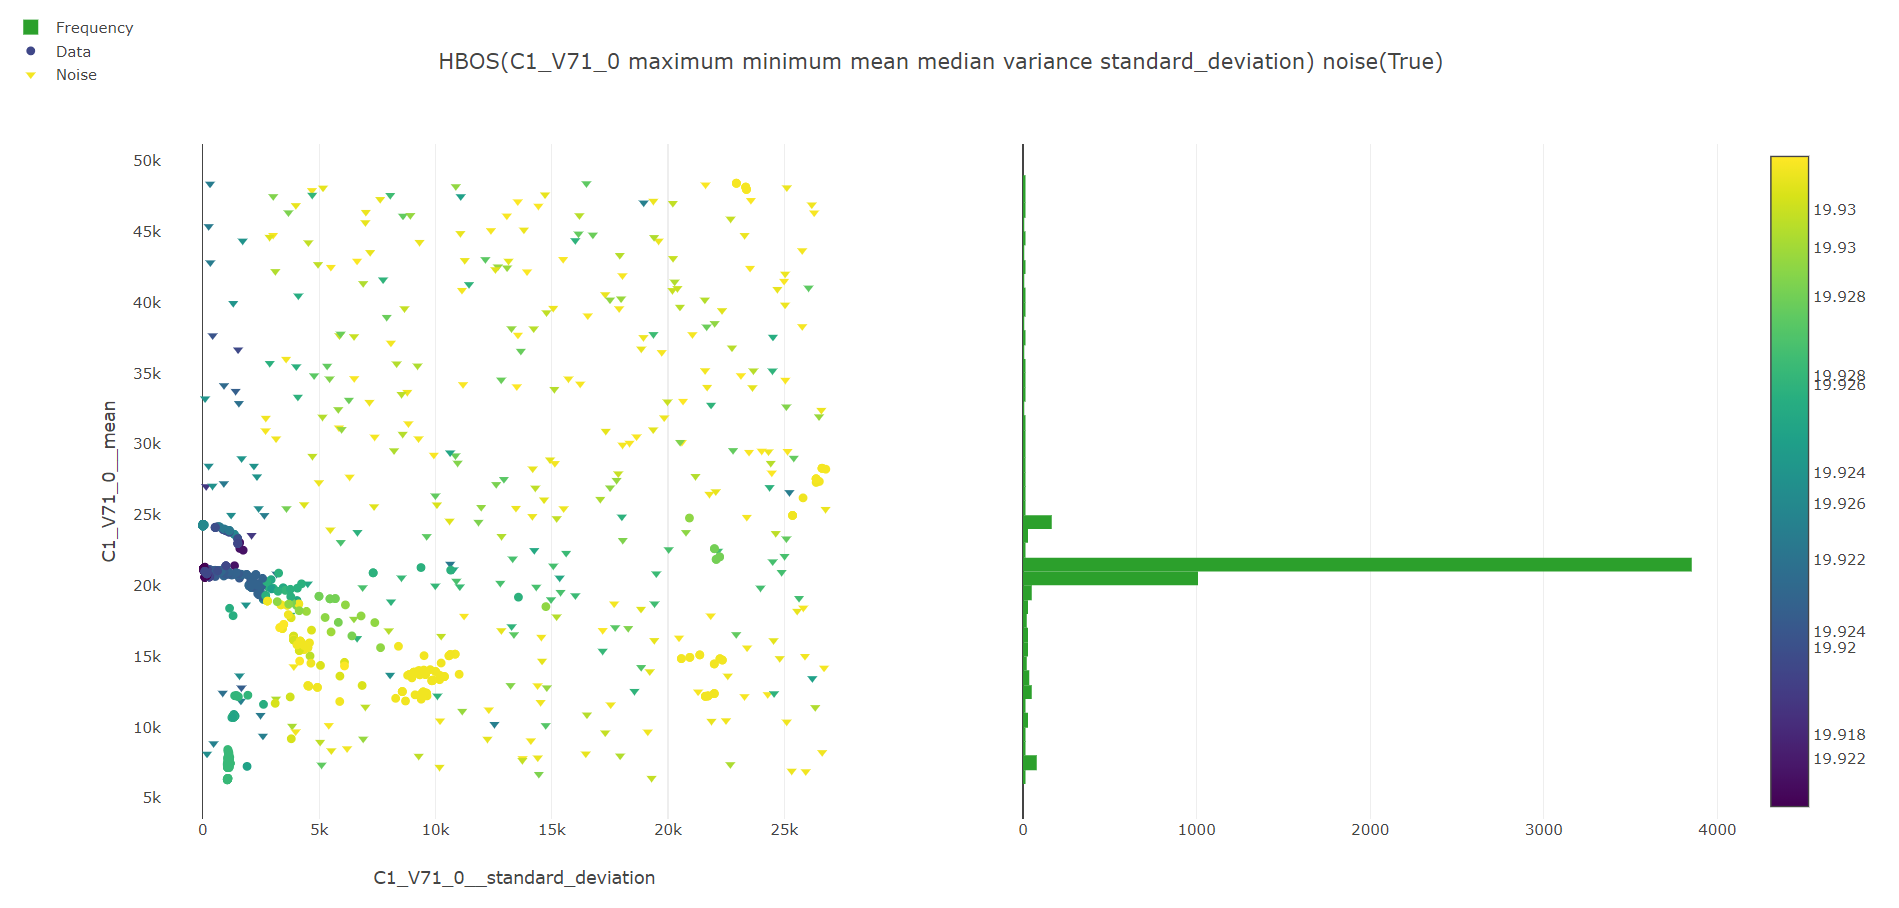
\includegraphics[width=\textwidth]{figures/vis3}
	\caption[Grafico dello score dei punti e del rumore usando HBOS e la variabile C1\_V71\_0]{Grafico dello score dei punti e del rumore usando HBOS e la variabile C1\_V71\_0. I punti verso il giallo sono più probabilmente outlier, mentre i punti verso il blu scuro sono più probabilmente inlier.
		
		\label{fig:vis3}}
\end{figure}


\subsection{Visualizzazione degli outlier con rumore a cluster}

Nella figura \ref{fig:vis4} il grafico mostra la classificazione degli outlier con l'aggiunta del rumore in 5 cluster casuali. Questa immagine conferma le conclusioni tratte alla fine della sezione \ref{AddestramentoEConfronto}, ovvero i cluster sono troppo distanti dai dati originali e troppo poco densi per poter confondere gli algoritmi di apprendimento. 

\begin{figure} [H]
	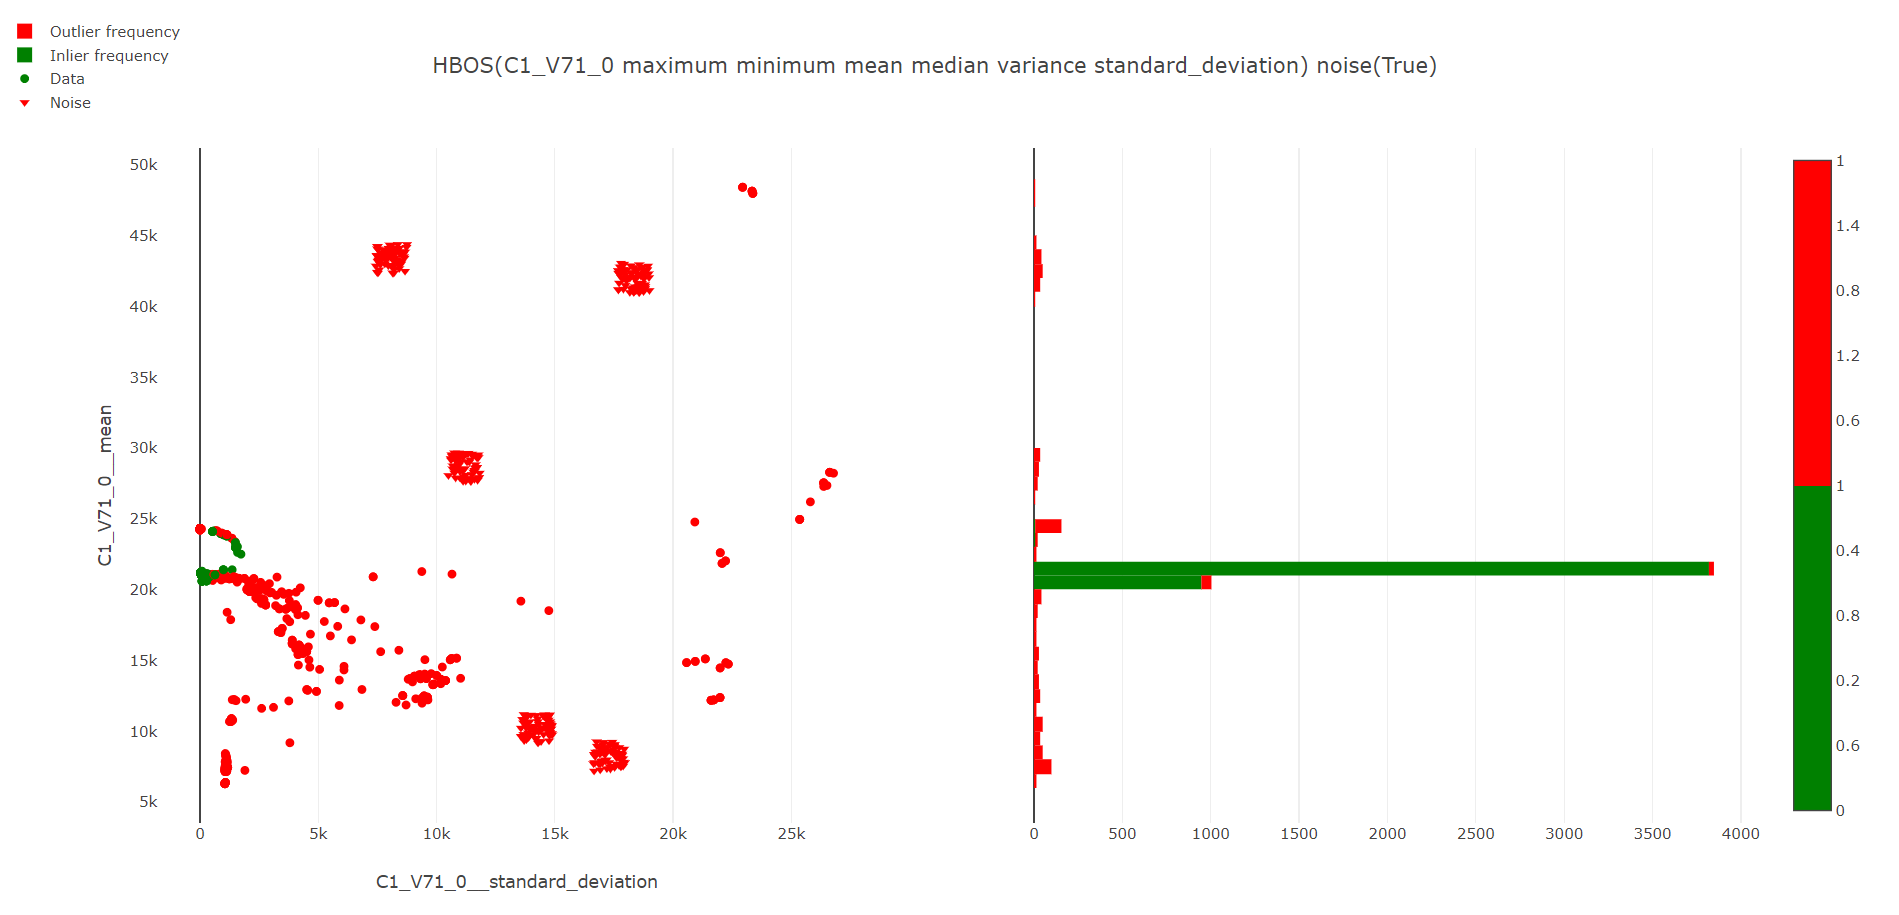
\includegraphics[width=\textwidth]{figures/vis4}
	\caption[Grafico degli outlier con aggiunta di rumore a cluster usando HBOS e la variabile C1\_V71\_0]{Grafico degli outlier con aggiunta di rumore in 5 cluster casuali usando HBOS e la variabile C1\_V71\_0. In rosso gli outlier, in verde gli inlier.
		
		\label{fig:vis4}}
\end{figure}


\subsection{Visualizzazione della decision surface}
La decision surface divide la superficie in più zone, ognuna delle quali rappresenta la probabilità che un punto in quella zona sia un'anomalia. Come si vede in figura \ref{fig:decision_surface} le zone rosse indicano che un punto in quelle zone è molto probabilmente un'anomalia, punti nelle zone blu sono comunque classificati come outlier ma è probabile che non lo siano. 

La linea tratteggiata rossa rappresenta la "decision boundary" ovvero il perimetro all'interno del quale i punti sono classificati come inlier. Per visualizzare meglio la decision surface, in figura \ref{fig:decision_surface} viene mostrata solo una parte del set di dati usato. 

Inoltre si possono notare le differenze tra i cinque algoritmi in base alle decision surface che generano, ad esempio PCA estrae le due componenti principali e forma quindi un ovale, oppure HBOS genera una superficie squadrata perché considera gli istogrammi di frequenza dei due assi.

\begin{figure} [H]
	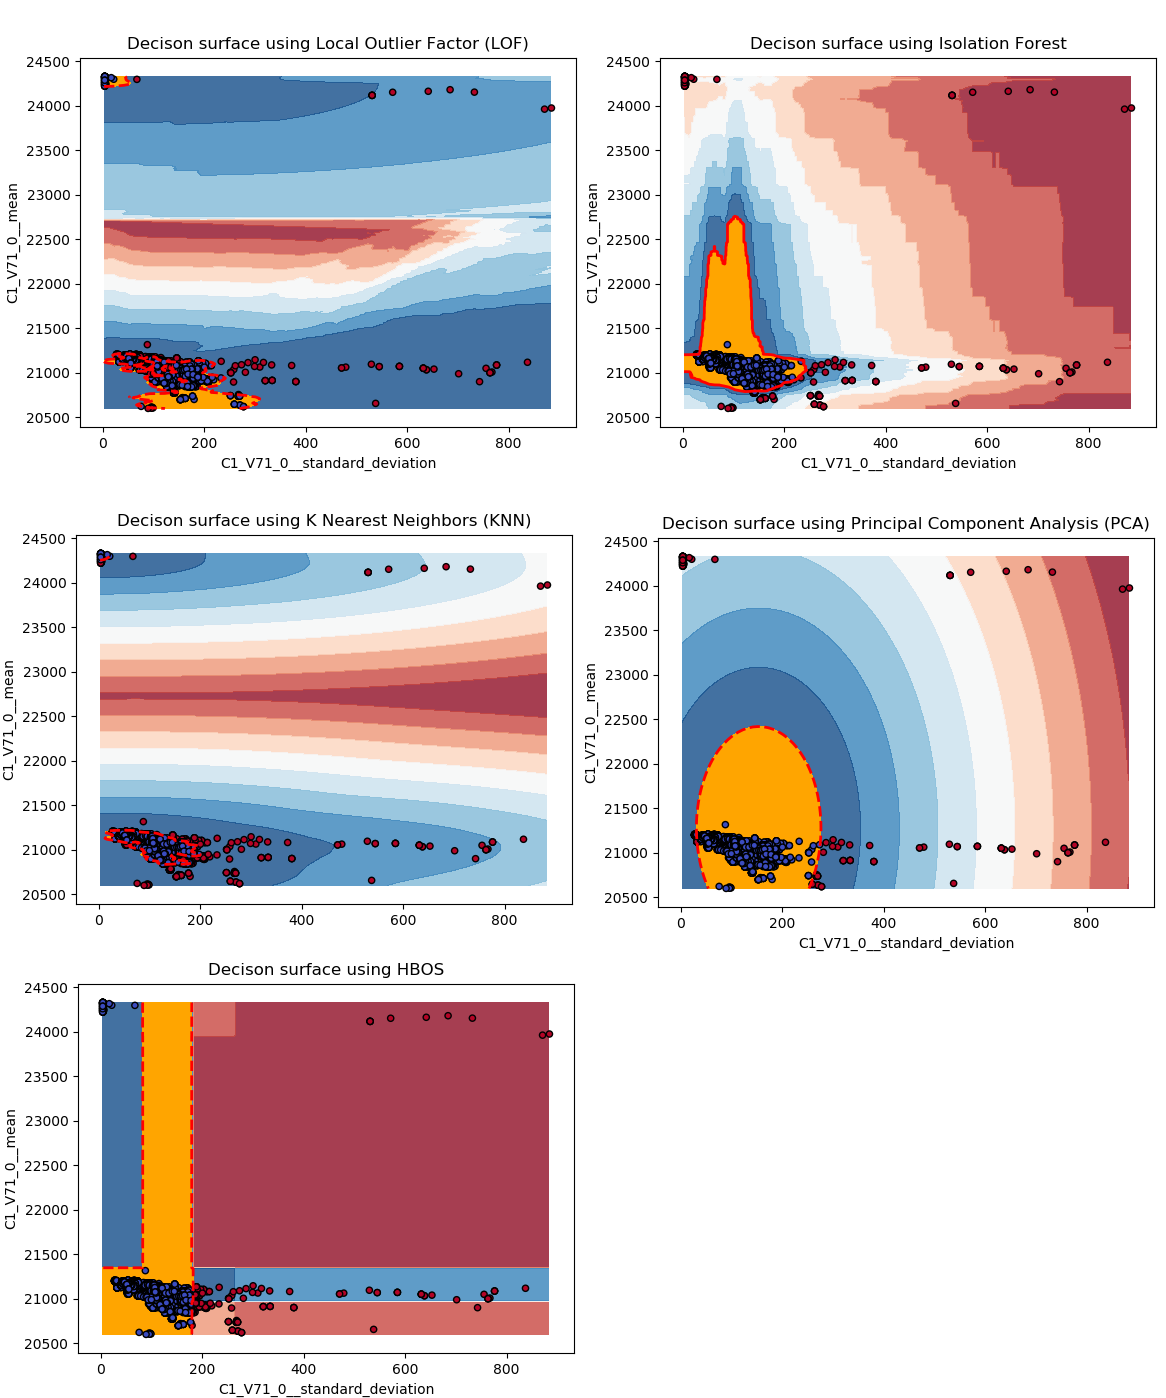
\includegraphics[width=\textwidth]{figures/decision_surface}
	\caption[Decision surface degli algoritmi]{Decision surface dei cinque algoritmi, le zone rosse indicano che un punto in quelle zone è molto probabilmente un'anomalia, punti nelle zone blu sono comunque classificati come outlier ma è meno probabile che lo siano. I punti all'interno della linea tratteggiata rossa sono inlier.
		
		\label{fig:decision_surface}}
\end{figure}


%!TEX root = ../dissertation.tex
\chapter{Conclusioni}
\label{conclusion}

Lo stage si è svolto seguendo ogni settimana il piano di lavoro descritto nella sezione \ref{PianoDiLavoro}. Il lavoro è stato ben pianificato dal tutor aziendale e in ogni parte del progetto non ci sono stati ritardi nelle consegne del software o dei documenti. Il tempo, infatti, è stato sufficiente anche per studiare le tecnologie utilizzate e le possibili alternative, per poterle confrontare ed effettuare la scelta migliore. Il codice segue i vincoli di stile scelti ed è stato progettato per essere il più possibile scalabile ed estendibile. Ogni classe e metodo è stato commentato, dai commenti è stata generata automaticamente la documentazione attraverso Sphinx. Grazie ai documenti prodotti e alla documentazione del codice il progetto è facilmente utilizzabile ed estendibile dai ricercatori dell'azienda. Tutti i requisiti individuati sono stati soddisfatti.

Le ultime due settimane, come da piano di lavoro, sono servite come introduzione all'intelligenza artificiale ed è stato possibile studiare vari algoritmi di feature extraction e di anomaly detection. Per addestrare un algoritmo di machine learning in grado di effettuare anomaly detection efficacemente su un problema ampio e complesso come la misurazione dei flussi multifase\cite{multiphaseIntroduction}, sarebbero stati necessari mesi di studio e di lavoro aggiuntivo, chiaramente fuori dai tempi dello stage. I risultati ottenuti sono comunque un ottimo studio di fattibilità sul problema, anche se sono state utilizzate solo alcune delle variabili lette dai sensori e non sono stati ancora tenuti in considerazione i possibili regimi di scorrimento del flusso descritti in sezione \ref{multiphaseflowmeter}. 

Un approccio diverso al problema potrebbe essere effettuare dei test in cui viene manomesso o modificato intenzionalmente il Multiphase Flow Meter per simulare un'anomalia. In questo modo i dati possono essere classificati come "normali" quando sono letti con il MPFM funzionante e come "anormali" quando sono letti con il MPFM modificato. Avere i dati già classificati permette di utilizzare algoritmi di machine learning basati sull'apprendimento supervisionato e ottenere un risultato probabilmente più preciso.


\addcontentsline{toc}{chapter}{References}
%\bibliographystyle{unstr}
\bibliography{references}
\cleardoublepage
\phantomsection
%\addcontentsline{toc}{chapter}{Acknowledgments}
%\acknowledgments


% \clearpage
% \bibliography{references}
% \addcontentsline{toc}{chapter}{References}
% \bibliographystyle{apalike2}

% %!TEX root = ../dissertation.tex
\newpage

% If you do want an image in the colophon:
\begin{figure}
  \vspace{20pt}
  \centering
  \hspace*{-32pt}
  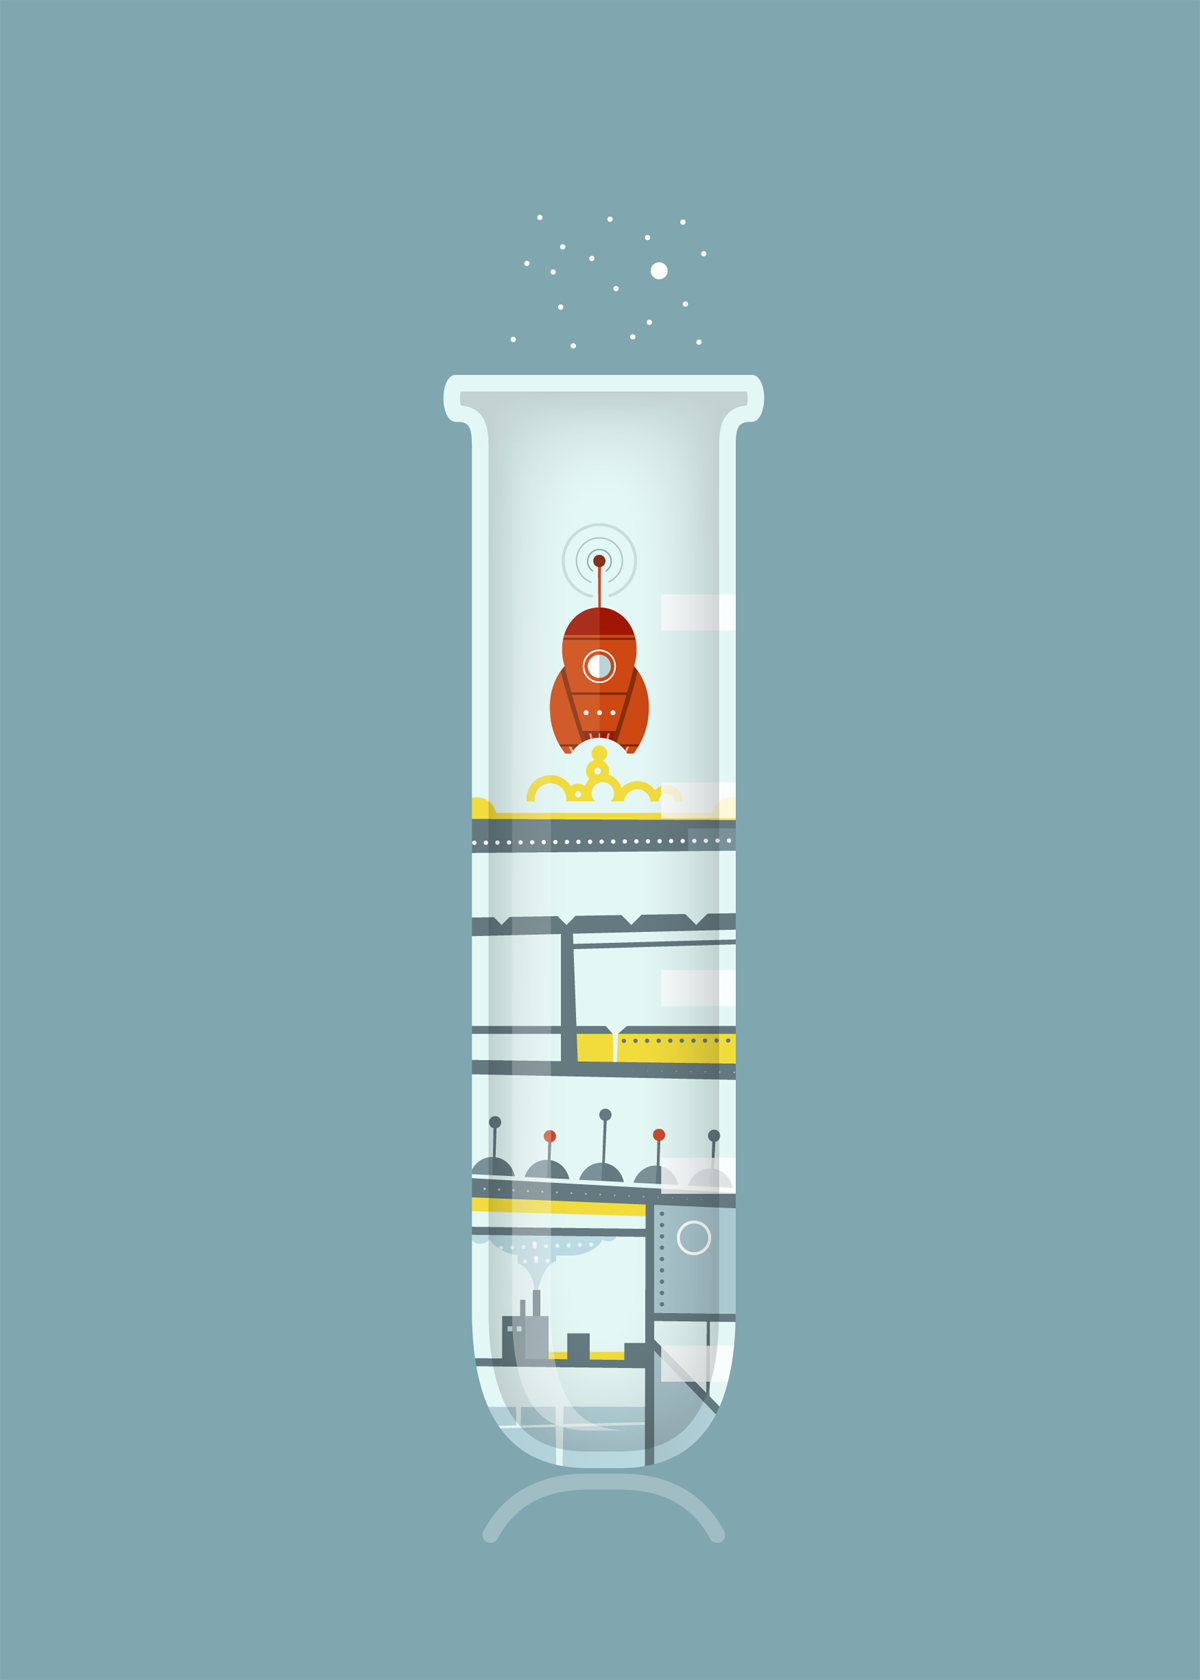
\includegraphics[width=0.42\textwidth]{endmatter/colophon.png}
\end{figure}

% If you don't want an image in the colophon:
% \vspace*{200pt}

\begin{center}
\parbox{200pt}{\lettrine[lines=3,slope=-2pt,nindent=-4pt]{\textcolor{SchoolColor}{T}}{his thesis was typeset} using \LaTeX, originally developed by Leslie Lamport and based on Donald Knuth's \TeX. The body text is set in 11 point Egenolff-Berner Garamond, a revival of Claude Garamont's humanist typeface. The above illustration, \textit{Science Experiment 02}, was created by Ben Schlitter and released under \href{http://creativecommons.org/licenses/by-nc-nd/3.0/}{\textsc{cc by-nc-nd 3.0}}. A template that can be used to format a PhD dissertation with this look \textit{\&} feel has been released under the permissive \textsc{agpl} license, and can be found online at \href{https://github.com/suchow/Dissertate}{github.com/suchow/Dissertate} or from its lead author, Jordan Suchow, at \href{mailto:suchow@post.harvard.edu}{suchow@post.harvard.edu}.}
\end{center}


\end{document}
